\documentclass{sn-jnl}

\usepackage{enumitem}
\usepackage{graphicx}
\usepackage{subcaption}
\usepackage{amsmath}
\usepackage{amssymb}
\usepackage{amsfonts}
\usepackage{dsfont}
\usepackage{mathtools}
\usepackage{mathrsfs}
\usepackage{algorithm}
\usepackage{algpseudocode}
\usepackage{tcolorbox}
\usepackage{float}
\usepackage[numbers]{natbib}
\newtheorem{assumption}{Assumption}
\newtheorem{remark}{Remark}
\newtheorem{example}{Example}
\newtheorem{theorem}{Theorem}
\newcommand{\indep}{\mathrel{\perp\!\!\!\perp}}

\begin{document}

\title{A General Framework for Joint Multi-State Models}

\author[1]{\fnm{Félix} \sur{Laplante}}\email{math.felixlaplante@proton.me}
\author*[2]{\fnm{Christophe} \sur{Ambroise}}\email{christophe.ambroise@univ-evry.fr}

\affil*[1]{\orgdiv{MaIAGE}, \orgname{Université Paris-Saclay, INRAE},
    \orgaddress{\country{France}}}
\affil[2]{\orgdiv{Laboratoire de Mathématiques et Modélisation d'Évry (LaMME)},
    \orgname{Université Paris-Saclay, CNRS, Univ Évry},
    \orgaddress{\country{France}}}

\abstract{
    Conventional joint modeling approaches generally characterize the relationship between longitudinal biomarkers and discrete event occurrences within terminal, recurring or competing risk settings, thereby offering a limited representation of complex, multi-state trajectories.

    We propose a general multi-state joint modeling framework that unifies longitudinal biomarker dynamics with multi-state time-to-event processes defined on arbitrary directed graphs. The proposed framework also accommodates nonlinear longitudinal submodels and scalable inference via stochastic gradient descent. This formulation encompasses both Markovian and semi-Markovian transition structures, allowing recurrent cycles and terminal absorptions to be naturally represented. The longitudinal and event processes are linked through shared latent structures within nonlinear mixed-effects models, extending classical joint modeling formulations.

    We derive the complete likelihood, model selection criteria, and develop scalable inference procedures based on stochastic gradient descent to enable high-dimensional and large-scale applications. In addition, we formulate a dynamic prediction framework that provides individualized state-transition probabilities and personalized risk assessments along complex event trajectories.

    Through simulation and application to the PAQUID cohort, we demonstrate accurate parameter recovery and individualized prediction.
}

\keywords{joint modeling, multi-state processes, longitudinal
    data, survival analysis, stochastic gradient
    descent, dynamic prediction}

\maketitle

\section{Introduction} \label{sec:introduction}

Joint modeling of longitudinal and time-to-event data has become an essential tool of modern biostatistics \citep{papageorgiou2019overview}, particularly for dynamic prediction in clinical applications. Classical joint models typically couple a longitudinal biomarker process with a single time-to-event outcome \citep{rizopoulos2012joint}, allowing for the integration of biological knowledge and individual heterogeneity via shared latent structures. However, many real-world processes involve multiple possible outcomes, intermediate stages, or recurrent events, which cannot be fully captured by a single-event framework \citep{KrolMauguen2017}. To address these limitations, specialized frameworks have been developed to handle competing risks and recurrent events. However, these remain constrained to specific event types and fail to accommodate more general multi-state transitions. In such settings, multi-state models provide a more general and flexible approach \citep{ferrer2016joint, you2024joint}.

Multi-state models represent an overall joint process of clinical course as a series of discrete stages or health states that occur sequentially \citep{lovblom2024modeling}. In biostatistics, these models are widely used for survival and reliability analysis, allowing for a richer and more accurate representation by capturing alternative paths to an event of interest, intermediate events, and progressive disease. Key components of multi-state models include transition intensity functions, which denote the instantaneous risk of moving from one state to another, and transition probability functions, which describe the probability of transition over longer intervals. Often, these models assume the Markov property, where future transitions depend only on the current state, simplifying the transition intensity functions \citep{asanjarani2022estimation}. This assumption can be relaxed by adopting a semi-Markov formulation, in which the transition probabilities depend not only on the current state but also on the sojourn time, effectively resetting the time scale after each transition.

The link between multi-state models and joint models arises when a multi-state process is integrated as a component within a broader joint modeling framework. While multi-state models, such as those described in the ``sequential state framework'' primarily focus on movements between discrete states, joint models operate under a ``parallel trajectory framework'' that combines a longitudinal process with a time-to-event process.

The model proposed by Ferrer et al.~\citep{ferrer2016joint} exemplifies this link by presenting a joint model for a longitudinal process (e.g., Prostate-Specific Antigen (PSA) measurements) and a multi-state process (e.g., clinical progressions in prostate cancer). These two sub-models are interconnected by shared random effects, allowing the model to account for the correlation between a continuous longitudinal biomarker trajectory and acyclic discrete transitions between health states. Specifically, the previously proposed mechanism \citep{ferrer2016joint, you2024joint} is based on binary censoring indicators for each state, implying that any given state can be entered at most once, therefore precluding the modeling of recurrent events.

The model we propose operates on an arbitrary directed graph, enabling representation of complex state transitions and recurrent events. We derive the complete likelihood for the nonlinear joint model, introduce an efficient stochastic approximation inference method, and develop dynamic prediction tools. To illustrate its practical relevance, we conduct both a simulation study and a synthetic biomedical case study.

This paper is organized as follows. Section~\ref{sec:background} reviews the background on multi-state and joint modeling frameworks. Section~\ref{sec:model} introduces the proposed general multi-state joint modeling framework, detailing the likelihood formulation and proposed model selection criteria. Section~\ref{sec:inference} describes the stochastic-gradient–based inference algorithm, while Section~\ref{sec:prediction} presents the dynamic prediction framework. Section~\ref{sec:experiments} reports simulation experiments that assess parameter recovery and convergence properties of the proposed model, whereas Section~\ref{sec:paquid} applies the framework to data from the PAQUID cohort. Finally, Section~\ref{sec:conclusion} concludes with perspectives and future research directions.

\section{Background} \label{sec:background}

Joint modeling of longitudinal and time-to-event data provides a unified statistical framework to analyze the interplay between continuous biomarker dynamics and event occurrence processes. In its classical form, this framework couples a mixed-effects model describing individual biomarker trajectories with a survival model for event times \citep{rizopoulos2012joint}. Such models have become central in biomedical research, particularly for dynamic prediction and personalized risk assessment \citep{papageorgiou2019overview}. However, these traditional joint models generally focus either on a single terminal event, competing, or recurrent events, limiting their ability to represent more complex event histories that include intermediate, recurrent, or competing events. To address these limitations, multi-state extensions have been developed, providing a natural framework for describing transitions between multiple clinical or biological states over time \citep{ferrer2016joint, KrolMauguen2017}.

\subsection{Multi-State Markov Processes}

A \emph{multi-state stochastic process} is defined as a process $S(t)$ for $t \geq 0$, where $S(t)$ can take a finite number of values (states), often labeled $1, 2, \dots, p$. Quantities of interest typically include the probability of being in a certain state at a given time and the distribution of first passage times.

A \emph{Markov process} (or continuous-time Markov chain) is a
specific class of multi-state models in which future transitions between states \emph{depend only upon the current state}. This \emph{Markov property} means the process is \emph{memoryless}. A key consequence is that the duration spent in any state follows an \emph{exponential distribution}, implying a constant hazard rate for leaving that state \citep{jackson2011multi,putter2007competing}.

However, the Markov assumption can be unrealistic in many real-world applications. For example, in the study of human sleep stages, sojourn times often do not follow an exponential distribution \citep{dong2008non, roever2010statistical}, and in the case of chronic diseases such as AIDS, the risk of disease progression can depend on the time elapsed since infection \citep{andersen1999multi}. To address these limitations, \emph{semi-Markov processes} (SMPs) were introduced, which allow for arbitrary distributions of sojourn times while retaining the Markov property for the embedded discrete-time chain. This flexibility makes SMPs suitable for modeling complex disease progression and patient recovery scenarios \citep{putter2007competing}.

\subsection{Multi-State Semi-Markov Processes}

\emph{Multi-state semi-Markov processes} (MSMPs) offer a natural generalization by allowing the distribution of sojourn times to be arbitrary.

In an MSMP, the process is defined by a directed graph $G = (V, E)$,
where $V$ represents the set of states and $E$ the set of possible transitions. The transition intensities $\lambda_{k' \mid k}(t \mid t_0)$ from state $k$ to state $k'$ at time $t$, given entry time $t_0$, are therefore assumed to be non identically zero. The sojourn time in state $k$ is not restricted to an exponential distribution, allowing for more realistic modeling of the time spent in each state.

MSMPs have been widely applied in a range of disciplines. In reliability, they are used to model degradation and repair processes \citep{limnios2001semi}. In biomedical studies, they have proven useful for analyzing illness-death models or disease progression with non-exponential transitions \citep{commenges2006likelihood, fiocco2008modelling}. Applications in finance also exist, where semi-Markovian dynamics can model credit rating migrations or economic regimes \citep{luciano2006semi}. In these contexts, MSMPs retain the Markov property in the embedded jump chain while offering increased realism through flexible dwell time modeling.

From a methodological standpoint, MSMPs extend estimation strategies developed for Markov models, such as maximum likelihood or Bayesian inference, and can accommodate interval-censored or misclassified data \citep{frydman2005estimation}. This makes them a powerful and general tool for multi-state event history analysis.

While both joint models and multi-state models offer powerful tools, they primarily address different facets of disease progression and have complementary strengths. Multi-state models excel at understanding the sequence and timing of discrete events, while joint models are adept at modeling continuous biomarker trajectories and their associations with event outcomes for dynamic prediction. The complexity of real-world diseases often necessitates a more integrated approach that can leverage the strengths of both frameworks. For instance, in prostate cancer, multiple types of relapse may occur successively (a multi-state process), and their risk is influenced by the dynamics of longitudinal biomarkers like PSA.

\subsection{Joint Models and Multi-State Processes}

Previous research has initiated such integration, with models like the one proposed by Ferrer et al.~\citep{ferrer2016joint}, which combines a linear mixed sub-model for longitudinal data with a multi-state sub-model using shared random effects. This model enables the simultaneous analysis of \emph{repeated measurements of a biomarker} (the longitudinal process, e.g., PSA levels) and the \emph{times of transitions between multiple health states} (the multi-state process). It explicitly accounts for the link between these two correlated processes and uses information from the biomarker dynamics to explain or predict clinical progression events. The multi-state sub-model assumes a \emph{non-homogeneous Markov process} for the clinical progression, meaning that the future of the process depends only on the current state (Markov property) and the time elapsed since study entry (non-homogeneous property).

Although Ferrer et al.~\citep{ferrer2016joint} note that their joint modeling framework could be adapted to semi-Markov processes in other contexts, their primary application to prostate cancer progression assumes a non-homogeneous Markov multi-state process. However, this framework is not well suited for arbitrary transition patterns other than the ones modeled by DAGs.

While both joint models and multi-state models offer powerful tools for analyzing disease progression, they emphasize different aspects of the underlying process. Multi-state models capture the sequence and timing of discrete transitions between states, whereas joint models focus on the evolution of continuous longitudinal markers and their association with event risk. Existing joint multi-state models, such as that of Ferrer et al.~\citep*{ferrer2016joint}, are restricted to linear mixed-effects submodels and to acyclic Markov transition graphs, as their likelihood relies on a sequential factorization that is not valid when transitions form cycles. However, many biological processes involve cyclic or semi-Markov transitions and nonlinear biomarker dynamics. These cannot be handled by existing frameworks, motivating the present general formulation.

In contrast, many real-world processes—such as recurrent disease relapse or recovery—require more flexible representations involving nonlinear biomarker dynamics, semi-Markovian dependencies, and recurrent cycles. The next section introduces a general framework that integrates these features within a unified likelihood-based formulation, enabling efficient inference and dynamic prediction along complex event trajectories.

\section{A General Multi-State Joint Modeling Framework}

To address the limitations imposed by traditional joint modeling frameworks, we extend them to incorporate a multi-state process, thereby enabling a unified analysis of longitudinal biomarkers and discrete transitions between multiple health states.

The proposed model defines a joint process $\{Y_i(t), S_i(t)\}_t$, where $Y_i(t)$ denotes the longitudinal biomarker trajectory and $S_i(t)$ the multi-state event process. Both components are linked through shared latent structures, and the event process is represented on an arbitrary directed graph supporting both Markovian and semi-Markovian transition mechanisms.

\subsection{Notation Conventions}

Throughout this section, let $i \in \{1, \dots, n\}$ index $n \geq 1$ individuals, and let $t_{ij}$ denote the $j$-th observation time of individual $i$. The vector $Y_{ij} \in \mathbb{R}^d$ represents longitudinal biomarker measurements, and $X_i \in \mathbb{R}^p$ the associated covariates.  

The latent random effects $b_i \sim \mathcal{N}(0, Q)$ capture individual heterogeneity, and the subject-specific parameters are defined as $\psi_i \coloneqq f(\gamma, X_i, b_i)$. The set $\mathcal{H}_i(t) \coloneqq \{ (w, h(w, \psi_i)) : w \leq t \}$ represents the true underlying history of the longitudinal process up to time $t$. Correspondingly, $\mathcal{Y}_i(t)$ denotes the observed longitudinal history, and $\mathcal{S}_i(t)$ denotes the observed trajectory of the semi-Markovian dynamics.  

Transition times and states are denoted by $(T_{i\ell}, S_{i\ell}) \in \mathbb{R} \times E$, where $E$ is the space of admissible states, and are subject to right-censoring at time $C_i$. We define the index of the last observed transition before time $t$ as $m_i(t) \coloneqq \sup \{ \ell \geq 0 : T_{i\ell} \leq t \}$. The complete sequence of transition times and states for individual $i$ is denoted by $\mathcal{T}_i^*$, whereas $\mathcal{T}_i$ denotes the corresponding right-censored sequence.

\subsection{Extending Multi-State Joint Models} \label{sec:model}

The joint model proposed by Ferrer et al. \citep{ferrer2016joint} established a foundational link between longitudinal biomarkers and multi-state processes through shared random effects. However, their formalism relies on binary censoring indicators to characterize transitions, thereby inherently restricting the modeling framework to Directed Acyclic Graphs (DAGs) and excluding recurrent events. Indeed, the proposed model uses, for each state $k \in E$, a tuple $(T_k, \delta_k)$, where $T_k$ denotes the observed or censored time until leaving state $k$ and $\delta_k$ is an indicator equal to $1$ if the transition was observed and $0$ if the observation was censored (\textit{i.e.}, the transition was not observed). While this representation may be adequate for traditional joint models, it implicitly assumes that each state can be exited at most once and thus precludes cycles or repeated visits, making it unsuitable for a generalization to more complex multi-state processes.

To overcome this limitation, we present a new method based on arbitrary graph transitions. By shifting away from binary indicators toward a more flexible graph-theoretic specification, our approach accommodates complex disease trajectories, including recurrent events and cyclic transitions that cannot be captured within a DAG-based structure.

\subsubsection{Graph Structure}

Let $G = (V,E)$ be a directed graph, where $V = \{1, \dots, p\}$ denotes the set of states and $E \subseteq V \times V$ the set of admissible transitions. The graph encodes all possible paths of the multi-state process, allowing for competing, recurrent, or absorbing transitions. Figure~\ref{fig:state-graph} illustrates an example of a four-state model, including an absorbing state (Death). The corresponding adjacency matrix $A = (A_{kk'})_{1 \leq k, k' \leq p}$ satisfies $A_{kk'} = 1$ if $(k, k') \in E$ and $0$
otherwise.

\begin{figure}[H]
    \centering
    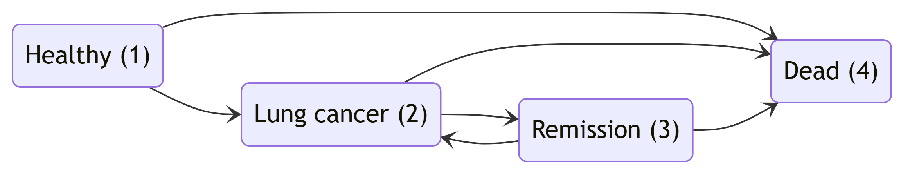
\includegraphics[width=0.8\textwidth]{diagrams/state-graph.pdf}
    \caption{Example of a 4-state transition graph $G = (V,E)$, including
        an absorbing state (4).}
    \label{fig:state-graph}
\end{figure}

Such a representation generalizes standard joint models, which can be recovered as special cases: single-event (linear chain), competing-risks (two absorbing transitions), or recurrent-event settings (cyclic transitions) as illustrated in Figure~\ref{fig:joint-models}.

\begin{figure}[H]
    \centering
    \begin{minipage}{0.31\textwidth}
        \centering
        \textbf{Standard Risk}
        \vspace{0.5em}
        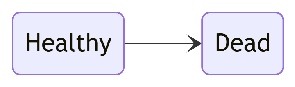
\includegraphics[width=0.85\textwidth]{diagrams/standard-graph.pdf}
    \end{minipage}
    \hfill
    \begin{minipage}{0.31\textwidth}
        \centering
        \textbf{Competing Risks}
        \vspace{0.5em}
        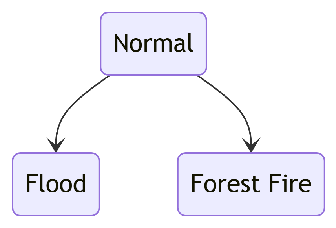
\includegraphics[width=0.9\textwidth]{diagrams/competing-graph.pdf}
    \end{minipage}
    \hfill
    \begin{minipage}{0.31\textwidth}
        \centering
        \textbf{Recurrent Risk}
        \vspace{0.5em}
        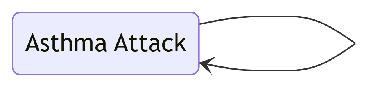
\includegraphics[width=\textwidth]{diagrams/recurrent-graph.pdf}
    \end{minipage}
    \caption{Illustration of classical joint modeling approaches: (left) standard risk, (middle) competing risks, and (right) recurrent risk.\label{fig:joint-models}}
\end{figure}

Such joint modeling offers a flexible framework that extends beyond classical approaches and is particularly useful in medical applications.

\subsubsection{Individual Trajectories}

Each individual $i \in \{ 1, \dots, n \}$ follows a latent trajectory
\[
    \mathcal{T}_i^* \coloneqq \big((T_{i0}, S_{i0}), (T_{i1}, S_{i1}), (T_{i2}, S_{i2}), \dots\big),
\]
where $T_{i\ell}$ denotes the $\ell$-th transition time and
$S_{i\ell} \in V$ the corresponding state. The observed trajectory is right-censored at time $C_i$, so that only $\mathcal{T}_i \coloneqq \{(T_{i\ell}, S_{i\ell}) : T_{i\ell} \leq C_i\}$ is observed. Between transitions, the state $S_i(t)$ is constant. Letting $m_i(t) \coloneqq \sup \{ \ell \geq 0 : T_{i\ell} \leq t \}$ be the index of the last observed transition before time $t$ and $m_i \coloneqq m_i(C_i)$, we thus assume that no further transitions occur for individual $i$ on the interval $(T_{im_i}, C_i]$. We also define $\mathcal{S}_i(t) \coloneqq \{ (w, S_i(w)) : w \leq t \}$ as the observed trajectory up to time $t$, which is equivalent to specifying all transition times and their corresponding states up to $t$, together with the time $t$ itself.


We emphasize once more that modeling the observed data solely as censored collections of transition times, as in Ferrer et al.~\citep{ferrer2016joint}, is not sufficient to represent such trajectories, since it implicitly restricts each state to be visited at most once and therefore rules out recurrent transitions.

The process is assumed to satisfy a (possibly time-inhomogeneous) semi-Markov property
\begin{equation} \label{ass:markov-property}
    \mathscr{L}\big((T_{i,\ell+1}, S_{i,\ell+1}) \mid \{(T_{i\ell'}, S_{i\ell'})\}_{\ell' \leq \ell}\big)
    = \mathscr{L}\big((T_{i,\ell+1}, S_{i,\ell+1}) \mid (T_{i\ell}, S_{i\ell})\big),
\end{equation}
which is relaxed compared to a stricter Markov property by allowing sojourn-time dependence.

\subsubsection{Transition Intensities and Survival Functions}

Although one could equivalently define intensities for all ordered pairs of states and set those corresponding to inadmissible transitions identically to zero, explicitly restricting attention to a graph of admissible transitions provides a clearer and more coherent representation of the underlying state dynamics.

For any admissible transition $(k, k') \in E$, let $\lambda_i^{k' \mid k}(t \mid t_0)$ denote the instantaneous risk of moving from $k$ to $k'$ at time $t$, given entry time $t_0$
\[
    \lambda_i^{k' \mid k}(t \mid t_0) \coloneqq \lim_{\delta \to 0^+}
    \frac{\mathbb{P}(T_{i,\ell+1} \leq t + \delta, S_{i,\ell+1}=k' \mid T_{i,\ell+1} > t, T_{i\ell}=t_0, S_{i\ell}=k)}{\delta}.
\]

The cumulative risk and the corresponding survival function are
\begin{align*}
     & \Lambda_i^{k' \mid k}(t \mid t_0) = \int_{t_0}^{t} \lambda_i^{k' \mid k}(w \mid t_0) \, dw, \\
     & \mathbb{P}(T_{i,\ell+1} > t \mid T_{i\ell}, S_{i\ell}) =
    \exp \left[-\sum_{s:(S_{i\ell},s)\in E}
        \Lambda_i^{s|S_{i\ell}}(t \mid T_{i\ell})\right].
\end{align*}

Conditional transition probabilities are
\[
    \mathbb{P}(S_{i,\ell+1} = k' \mid T_{i,\ell+1}, T_{i\ell}, S_{i\ell}) = \frac{\lambda_i^{k'|S_{i\ell}}(T_{i,\ell+1} \mid T_{i\ell})}{\sum_{s:(S_{i\ell},s)\in E}\lambda_i^{s|S_{i\ell}}(T_{i,\ell+1}\mid T_{i\ell})}.
\]

\subsection{Multi-State Joint Model Specification}

Omitting the implicit conditioning on the individual parameters and covariates for the sake of simple notation, the proposed multi-state joint model with a Gaussian prior and homoscedastic Gaussian noise is specified by
\[
\begin{cases}
    Y_{ij} = h(t_{ij}, \psi_i) + \epsilon_{ij}, \quad \epsilon_{ij} \sim \mathcal{N}(0, R), \\
    \lambda_i^{k' \mid k}\left( t \mid \mathcal{H}_i(t), \mathcal{S}_i(t) \right) = \lambda_0^{k' \mid k}(t \mid T_{im_i(t)}) \exp\big(\alpha^{k' \mid k} g^{k' \mid k}(t, X_i, \psi_i) + \beta^{k' \mid k} X_i\big), \\
    \psi_i = f(\gamma, X_i, b_i), \quad b_i \sim \mathcal{N}(0, Q).
\end{cases}
\]

Here, $h$ and $f$ define the nonlinear mixed-effects submodel,
$g^{k' \mid k}$ represents the link between biomarker dynamics and the transition intensity, and $\lambda_0^{k' \mid k}$ denotes the baseline hazard associated with transition $(k \to k')$. This structure extends the classical joint model to arbitrary directed graphs and to both Markovian and semi-Markov specifications. 

The coefficient $\alpha^{k' \mid k}$ quantifies the effect of the longitudinal biomarker dynamics on the instantaneous risk of transitioning from state $k$ to state $k'$. More concretely, for a one-unit increase in $g^{k' \mid k}(t,X_i,\psi_i)$ (holding other covariates constant), the hazard ratio for transition $(k \to k')$ is $\exp(\alpha^{k' \mid k})$. Likewise, $\beta^{k' \mid k}$ represents the effect of baseline (or time-varying) covariates $X_i$ on that same transition: a one-unit increase in a covariate $X_{ij}$ multiplies the hazard by $\exp(\beta^{k' \mid k}_j)$. Thus, $\alpha^{k' \mid k}$ captures the degree to which the biomarker trajectory (via its latent parameter $\psi_i$ or function $g^{k' \mid k}$) influences the transition risk, while $\beta^{k' \mid k}$ captures the direct effect of covariates on that transition’s risk, beyond the biomarker pathway.

\subsubsection{Model Variants}

Two baseline hazard conventions are common and can be specified as
\[
    \lambda_0^{k' \mid k}(t \mid T_{im_i(t)}) =
    \begin{cases}
        \lambda_0^{k' \mid k}(t - T_{im_i(t)}) & \text{(clock reset)},   \\
        \lambda_0^{k' \mid k}(t)               & \text{(clock forward)}.
    \end{cases}
\]

The \emph{clock-reset} form models risk as a function of time spent in the current state, whereas the \emph{clock-forward} form measures risk with respect to global time since study entry.

\subsubsection{Likelihood Formulation}

To derive the marginal likelihood, we decompose the joint distribution of the longitudinal and multi-state processes under a set of standard conditional independence assumptions detailed in Table~\ref{ass:likelihood} below.

\begin{tcolorbox}[title=\textbf{Assumptions for Likelihood Factorization}, colback=gray!4!white,colframe=gray!60!black,sharp corners,boxrule=0.5pt] \label{ass:likelihood}
    \textbf{A. Latent-level independence}
    \vspace{-1em}
    \begin{enumerate}[label=\textbf{A\arabic*.}, leftmargin=3em]
        \item Random effects $(b_i)_i$ are mutually independent across individuals.
    \end{enumerate}
    \vspace{-0.5em}
    \textbf{B. Conditional independence within individuals}
    \vspace{-1em}
    \begin{enumerate}[label=\textbf{B\arabic*.}, leftmargin=3em]
        \item Longitudinal observations $(Y_{ij})_{ij}$ are mutually independent given $b_i, X_i$.
        \item Trajectories $(\mathcal{T}_i^*)_i$ are mutually independent given $b_i, X_i$.
        \item Conditional on $b_i, X_i$, the longitudinal and event processes are mutually independent.
    \end{enumerate}
    \vspace{-0.5em}
    \textbf{C. Censoring and process assumptions}
    \vspace{-1em}
    \begin{enumerate}[label=\textbf{C\arabic*.}, leftmargin=3em]
        \item[\textbf{C1.}] Censoring times $(C_i)_i$ are mutually independent and noninformative, \textit{i.e.} $C_i \indep (Y_i, \mathcal{T}_i^*) \mid b_i, X_i$.
        \item[\textbf{C2.}] Conditionally on $b_i, X_i$, event trajectories satisfy the semi-Markov property~\ref{ass:markov-property}: $p(\mathcal{T}_i^* \mid b_i, X_i) = \prod_{\ell \geq 0} p\left( (T_{i,\ell+1}, S_{i,\ell+1}) \mid T_{i\ell}, S_{i\ell}, b_i, X_i \right)$.
    \end{enumerate}
\end{tcolorbox}

These grouped assumptions mirror those used in classical joint modeling \citep{rizopoulos2012joint} and multi-state survival analysis \citep{putter2007competing}: independence across subjects, the conditional independence structure linking the longitudinal and event submodels through shared random effects, noninformative censoring, and semi-Markovian dynamics.

\bigbreak

Let $\theta \coloneqq (\gamma, Q, R, \alpha, \beta)$ denote the vector of model parameters. For subject $i \in \{ 1, \dots, n \}$, we observe the longitudinal measurements $Y_i = (Y_{i1}, \dots, Y_{in_i})$ and the event trajectory $\mathcal{T}_i = \{ (T_{i\ell}, S_{i\ell})_{0 \leq \ell \leq m_i} \}$. The joint likelihood then factorizes as
\[
    p(Y_i, \mathcal{T}_i \mid X_i, C_i, \theta) = \int p(Y_i \mid b_i, X_i, \theta) \, p(\mathcal{T}_i \mid b_i, X_i, C_i, \theta) \, p(b_i \mid \theta) \, db_i.
\]

This formulation generalizes the joint likelihoods of \citet{wulfsohn1997joint} and \citet{ferrer2016joint} to arbitrary multi-state event structures. Each part can then be explicitly expressed using Assumptions~\ref{ass:likelihood}, yielding an expression very similar to that obtained by \citet{rizopoulos2012joint}.

\begin{description}
    \item[\textnormal{\textbf{Prior likelihood:}}]
        \[
            p(b_i \mid \theta) = \frac{(2 \pi)^{-q/2}}{\det(Q)^{1/2}}
              \exp\left(-\tfrac{1}{2} b_i^T Q^{-1} b_i \right),
        \]

    \item[\textnormal{\textbf{Longitudinal likelihood:}}]
        \begin{align*}
           &p(Y_i \mid b_i, X_i, \theta) = \prod_{j = 1}^{n_i} \frac{(2 \pi)^{-d/2}}{\det(R)^{1/2}} \exp\left(-\tfrac{1}{2} \left(Y_{ij} - h(t_{ij}, \psi_i)\right)^T
          R^{-1} \left(Y_{ij} - h(t_{ij}, \psi_i)\right)\right), \\
           &\text{with } \psi_i = f(\gamma, X_i, b_i).
        \end{align*}

    \item[\textnormal{\textbf{Semi-Markov likelihood:}}]
          \begin{equation}
              \begin{aligned}
                  p(\mathcal{T}_i \mid b_i, X_i, C_i, \theta) = &\prod_{l=0}^{m_i-1} p\left((T_{i(l+1)}, S_{i(l+1)}) \mid
                  b_i, X_i, (T_{il}, S_{il}), \theta\right) \\
                  &\exp\left(-\sum_{s : \, (S_{im_i}, s) \in E}
                  \Lambda_i^{s \mid S_{im_i}} (C_i \mid b_i, X_i, T_{im_i}, \theta)\right).
              \end{aligned}
              \label{ass:semi-markov}
          \end{equation}
\end{description}

The proof of the expression of the Semi-Markov likelihood
(\ref{ass:semi-markov}) is provided in Appendix
\ref{sec:proof-semi-markov}.

\bigbreak

The likelihood factorization above is valid and forms the basis for scalable inference procedures described in Section~\ref{sec:inference}, leveraging the complete trajectory of biomarkers to refine predictions of transitions and survival \citep{de2010mstate}.

Moreover, here, we assume that the initial state $S_{i0}$ is observed. However, the framework could also incorporate a multinomial model for unobserved initial states \citep{yiu2018clustered}.

\subsection{Model Selection and Information Criteria}

To compare competing model specifications, we rely on information criteria based on the marginal likelihood as defined in Section~\ref{sec:inference}. The Akaike Information Criterion (AIC) \citep{akaike2003new} and the Bayesian Information Criterion (BIC) \citep{schwarz1978estimating} are standard tools. While the AIC relies on an asymptotically unbiased estimator of the $\log$-likelihood, the BIC aims to identify the true model with high probability as the sample size grows.

The Akaike Information Criterion is computed as follows
\[
    \mathrm{AIC} \coloneqq -2 \log \mathcal{L}_\text{marginal}(\hat{\theta}; X, Y, \mathcal{T}, C) + 2 k,
\]
where $k$ is the number of parameters, and $\hat{\theta}$ is a maximizer of the marginal likelihood.

The Bayesian Information Criterion is similarly defined but imposes a stronger penalty for model complexity, growing in $\log n$ where $n$ is the number of observations. Particularly in the context of mixed effects models, and even more so for multi-state joint models, the number of observations $n$ may vary from one definition to another, either the total number of repeated measurements or the number of individuals \citep{delattre2014note}. To alleviate this problem, we recall the derivation of the BIC from the Laplace approximation \citep{lebarbier2006introduction}. For a prior distribution $\pi$ on a set of models $\mathcal{M}$, the Laplace approximation yields, up to constant terms (which could also be included to improve the approximation), the approximation of the posterior probability given observed data $x$ defined in Section~\ref{sec:inference} reads
\[
    \forall m \in \mathcal{M}, \, \log p(x \mid m) \approx \log \mathcal{L}_\text{marginal}(\hat{\theta}; x) - \frac{1}{2} \log \det(-H_{\hat{\theta}}),
\]
where $H_{\hat{\theta}}$ denotes the Hessian matrix of the marginal $\log$-likelihood evaluated at the Maximum Likelihood Estimator (MLE). Then, under standard regularity conditions that allow differentiation and integration to be interchanged twice, we have that
\[
    -\frac{1}{n} H_{\hat{\theta}} \overset{\mathbb{P}}{\to} \mathcal{I}(\hat{\theta}),
\]
where $\mathcal{I}(\hat{\theta})$ denotes the Fisher Information Matrix \citep{casella2001theory}. Given a reliable estimate $\widehat{\mathcal{I}}(\hat{\theta})$ of the Fisher Information Matrix (see, e.g., \citet{delattre2023computing}), we can then approximate the BIC by substituting this estimate
\[
    \forall m \in \mathcal{M}, \, \log p(x \mid m) \approx \log \mathcal{L}_\text{marginal}(\hat{\theta}; x) - \frac{1}{2} \log \det \hat{\mathcal{I}}_n(\hat{\theta}),
\]
where $\hat{\mathcal{I}}_n(\hat{\theta}) \coloneqq n \, \hat{\mathcal{I}}(\hat{\theta})$, which in practice corresponds to the matrix readily computed by our software. 

Thus, our BIC criterion can be written as
\[
\mathrm{BIC}_\mathcal{I} \coloneqq -2 \log \mathcal{L}_\text{marginal}(\hat{\theta}; x) + \log \det \hat{\mathcal{I}}_n(\hat{\theta}).
\]

In both cases, one should aim to minimize the chosen criterion.

\section{Statistical Inference} \label{sec:inference}

The estimation of model parameters $\theta = (\gamma, Q, R, \alpha, \beta)$ relies on two likelihood formulations: the complete-data likelihood $\mathcal{L}_{\text{complete}}$, which includes latent variables, and the marginal likelihood $\mathcal{L}_\text{marginal}$, obtained by integrating them out
\[
    \mathcal{L}_\text{marginal}(\theta ; X, Y, \mathcal{T}, C) = \int \mathcal{L}_\text{complete}(\theta; X, Y, \mathcal{T}, C, b) \,db,
\]
where
\[
    \mathcal{L}_\text{complete}(\theta  ; X, Y, \mathcal{T}, C, b) = \prod_{i=1}^n p(Y_i \mid b_i, X_i, \theta) \, p(\mathcal{T}_i \mid b_i, X_i, C_i, \theta) \, p(b_i \mid \theta).
\]

It is to be noted that this integral is typically intractable in closed form due to the nonlinear nature of the model. Several optimization methods adapted from the nonlinear mixed-effects literature can be applied, including Stochastic EM \citep{kuhn2004coupling}, Laplace approximation \citep{wolfinger1993laplace} and Gauss--Hermite quadrature, alongside MCMC-based approximations such as Metropolis--Hastings \citep{hastings1970monte} and Hamiltonian Monte Carlo \citep{neal2011mcmc}. These strategies are implemented in software such as \texttt{JMBayes} \citep{jmbayes22024,rizopoulos2020package}.

Another approach requiring mild regularity assumptions on the $\log$ marginal likelihood, but without the need for the model to belong in the exponential family, is to consider a stochastic gradient ascent scheme \citep{caillebotte2025estimation, baey2023efficient} using Fisher's identity and following the Robbins-Monro procedure \citep{robbins1951stochastic}.

Under interchangeability of integral and differentiation, setting $x \coloneqq (X, Y, \mathcal{T}, C)$ for convenience, the Fisher identity writes
\[
    \nabla_\theta \log \mathcal{L}_\text{marginal}(\theta ; x) = \mathbb{E}_{b \sim p(\cdot \mid x, \theta)} \left(\nabla_\theta \log \mathcal{L}_{\text{complete}}(\theta ; x, b)\right).
\]

This expectation is approximated using Monte Carlo samples from the posterior $p(\cdot \mid x, \theta)$, avoiding the need to evaluate the intractable marginal likelihood
$\mathcal{L}_\text{marginal}(\theta; x)$. This formulation naturally supports stochastic gradient ascent with MCMC-based posterior sampling and is amenable to minibatch parallelization across individuals, ensuring the convergence to a critical point. The update rule is described in Algorithm~\ref{alg:sgd}.

\begin{algorithm}[H]
    \caption{Stochastic gradient ascent model inference}
    \label{alg:sgd}

    \begin{algorithmic}[1]
        \algrenewcommand\algorithmicrequire{\textbf{Input:}}
        \Require data $x$; initial parameter $\theta^{(0)}$; step sizes $(\eta_t)_{t \geq 0}$ with $\sum_t \eta_t = +\infty$, $\sum_t \eta_t^2 < +\infty$; batch size $K$; sampler $p^{\mathrm{MCMC}}$; stopping criterion.
        \Statex
        \State $t \gets 0$
        \While{not converged}
        \State Draw $b_k \sim p(\cdot \mid x, \theta^{(t)}) \approx p^\text{MCMC}$.
        \State $\theta^{(t+1)} \gets \theta^{(t)} + \frac{\eta_t}{K} \sum_{k=1}^K \nabla_\theta \log \mathcal{L}_\text{complete} (\theta^{(t)} ; x, b_k)$.
        \State $t \gets t + 1$
        \EndWhile
        \State \Return $\hat{\theta}$
    \end{algorithmic}
\end{algorithm}

Preconditioning matrices may also be used, such as the Fisher Information Matrix in a natural gradient descent framework, or even specialized \emph{optimizers} such as Adam \citep{kingma2014adam}, NAdam \citep{dozat2016incorporating} or Adagrad \citep{duchi2011adaptive}. In particular, the Adam optimizer will later be used in our numerical experiments.

\section{Dynamic prediction} \label{sec:prediction}

The simulation of individual trajectories using Algorithm~\ref{alg:trajectory-sim} enables prediction in the multi-state joint modeling framework. Specifically, predictions are derived from simulated event trajectories, allowing for individualized risk assessment and forecasting of future states or event times based on a subject's observed biomarker and event history. This approach generalizes classical dynamic prediction by leveraging the rich structure of multi-state processes and the joint distribution of longitudinal and event data.

Let $i$ index a new individual. Suppose we are interested in some functional of the true (unobserved) future trajectory,
\[
    \chi^*(\mathcal{T}_i^*) \in \mathbb{Y},
\]
where $\mathbb{Y}$ is some generic space.

For example, one can think of the state taken by the individual $i$ at a time $u$. As is the case in traditional dynamic prediction however, we are only interested in predicting quantities or characteristics that depend on a yet unobserved \emph{future}, given prior information, \textit{i.e.} the trajectory $\mathcal{S}_i(t)$ up to some prediction time $t \leq u$ and observed longitudinal markers $\mathcal{Y}_i(t) \coloneq \{ (t_{ij}, Y_{ij}) : t_{ij} \leq t \}$. Contrary to (single transition) joint models, the conditional probability distribution on $(\mathbb{R} \times \mathcal{S})^\mathbb{N}$ cannot be analytically derived.

Nonetheless, as seen in Algorithm~\ref{alg:trajectory-sim}, we are able to accurately simulate each trajectory. Therefore, a single or double Monte Carlo estimation scheme may be devised under certain restrictions, where we estimate $\chi^*(\mathcal{T}_i^*)$ by its conditional expected value
\[
    \hat{\chi}_i^{(1)} \coloneqq \mathbb{E}\left(\chi^*(\mathcal{T}'_i) \mid \mathcal{Y}_i(t), \mathcal{S}_i(t), \hat{\theta}\right) \approx \frac{1}{B} \sum_{k=1}^B \chi^*(\mathcal{T}_i^{(k)}), \, \mathcal{T}_i^{(k)} \overset{\text{i.i.d.}}{\sim} \mathscr{L}(\mathcal{T}_i^* \mid \mathcal{Y}(t), \mathcal{S}_i(t), \hat{\theta}).
\]

Another approach from Bayesian perspective treats the model parameters $\theta$ as random variables by imposing a prior distribution together with the training data $\mathcal{D}_n$ \citep{rizopoulos2011dynamic}, and thus in this case our new estimator may be defined
\[
    \hat{\chi}_i^{(2)} \coloneqq \mathbb{E}_{\theta' \sim \mathscr{L}(\theta \mid \mathcal{D}_n)}\left(\mathbb{E}\left(\chi^*(\mathcal{T}'_i) \mid \mathcal{Y}(t), \mathcal{S}_i(t), \theta'\right)\right),
\]
and approximated by a double Monte Carlo accordingly.

\bigbreak

In general however, $\chi^*$ may very well depend on (countably) infinitely many transitions. As a result, since the proposed estimation relies on simulated samples, we require the quantity to depend only on a finite subset of transitions.

\begin{assumption} \label{ass:simulatable}
    There exists  $\chi: \bigcup_{n \geq 1} (\mathbb{R} \times V)^n \to \mathbb{Y}$ and $\tau_i$ a stopping time for the filtration $\mathcal{F}_{in} \coloneqq \sigma\left((T_{il}, S_{il})_{0 \leq \ell \leq n}\right)$ such that
    \[
        \begin{cases}
            \tau_i < +\infty \text{ a.s.}, \\
            \chi^*(\mathcal{T}_i^*) = \chi\left((T_{il}, S_{il})_{0 \leq \ell \leq \tau_i}\right)
        \end{cases}
    \]
\end{assumption}

Essentially, given Assumption~\ref{ass:simulatable}, with probability one we are guaranteed that the quantity of interest may be computed in a finite number of simulation steps. Indeed, the prediction algorithm for a single sample may be summarized as in Algorithm~\ref{alg:prediction}.

\begin{algorithm}[H]
    \caption{Prediction algorithm}
    \label{alg:prediction}
    \begin{algorithmic}[1]
        \algrenewcommand\algorithmicrequire{\textbf{Input:}}
        \Require $t \in \mathbb{R}$, a prediction time; $\mathcal{Y}(t)$ marker history; $\mathcal{T}_i$ trajectory up to time $t$; $\chi$ and stopping time $\tau_i$; $\hat{\theta}$ or $\mathscr{L}(\hat{\theta} \mid \mathcal{D}_n)$.
        \Statex
        \State $n \gets \mathrm{len}(\mathcal{T}_i)$
        \While{$n \leq \tau_i$}
        \State Append simulated $(T_{in}, S_{in})$ to $\mathcal{T}_i$
        \State $n \gets n + 1$
        \EndWhile
        \State \Return $\chi\left((T_{il}, S_{il})_{0 \leq \ell \leq \tau_i}\right)$
    \end{algorithmic}
\end{algorithm}

Numerous quantities of interest may be encompassed by this framework. We give multiple examples below. First, for a directed acyclic graph $G = (V, E)$, we define the \emph{depth} of $G$, denoted by $\operatorname{depth}(G)$, as the length of the longest directed path in $G$, that is,
\[
    \operatorname{depth}(G) \coloneqq \max_{(v_0, v_1, \dots, v_k)} k,
\]
where $(v_0, v_1, \dots, v_k)$ ranges over all directed paths in $G$.

\begin{example}[State at time $u$] \label{ex:state-at-time-u}
    Let $G = (V, E)$ be a finite directed acyclic graph, $u \in \mathbb{R}$ be a fixed time, and $\mathbb{Y} = V$ be the set of possible states. Let $\tau_i = \inf \{ n \in \mathbb{N}: T_{in} \geq u \text{ or } S_{in} \text{ is absorbing} \}$. Clearly, $\tau_i \leq \operatorname{depth}(G) < +\infty$. Then, take $\chi_u^*(\mathcal{T}_i^*) = S_{i\tau_i}$, which corresponds to the state of the individual $i$ at time $u$. In particular, if $V = \{ 0, 1 \}$ and $E = \{ (0, 1) \}$, we recover the special case used for survival probability estimation in standard joint models \citep{rizopoulos2011dynamic}.
\end{example}

\bigbreak

\begin{example}[Hitting time] \label{ex:hitting-time}
    Let $G = (V, E)$ be a finite directed acyclic graph, $\mathbb{A} \subseteq V$ a non-empty subset of states, and $\mathbb{Y} = \mathbb{R} \cup \{ +\infty \}$. For any two non-empty sets $\mathbb{A}, \, \mathbb{B} \subseteq V$, we note $\mathbb{A} \rightsquigarrow \mathbb{B}$ if there exists a path from $\mathbb{A}$ to $\mathbb{B}$ in $G$. Let $\tau_i = \inf \{ n \in \mathbb{N} : S_{in} \in \mathbb{A} \vee  \{ S_{in} \} \not \rightsquigarrow \mathbb{A} \}$. Then, $\tau_i \leq \operatorname{depth}(G) < +\infty$ and take $\chi_{\mathbb{A}}^*(\mathcal{T}_i^*) = T_{i\tau_i} + \mathds{1}_{\{ S_{i\tau_i} \} \not \rightsquigarrow \mathbb{A}} (+\infty)$ represents the hitting time for the set $\mathbb{A}$.
\end{example}

\bigbreak

In Example~~\ref{ex:state-at-time-u}, the stopping time $\tau_i$ captures the step at which the process for individual $i$ reaches or exceeds a given time $u$, or enters an absorbing state.
The resulting value $\chi^*(\mathcal{T}_i^*) = S_{i\tau_i}$ therefore represents the state of the individual at that specific time.

In Example~\ref{ex:hitting-time}, the stopping time $\tau_i$ corresponds to the first time the process reaches a target subset of states $\mathbb{A}$, or becomes unable to reach it in the future.
The associated value $\chi_{\mathbb{A}}^*(\mathcal{T}_i^*)$ thus represents the \emph{hitting time} of the set $\mathbb{A}$, which may be finite if $\mathbb{A}$ is reached, or $+\infty$ otherwise.

\bigbreak

Other practical applications may include finding the expected number of edges in some given trajectory, the number of times an individual has returned in a specific state, the expected time between transitions\dots

This simulation-based dynamic prediction framework generalizes classical approaches from single-event joint models to the multi-state context. It enables individualized forecasting of future state occupancy, event risks, sojourn times, and other clinically relevant outcomes, fully exploiting the subject's observed biomarker trajectory and event history. In Section~\ref{sec:paquid}, we demonstrate its application to forecasting dependency trajectories in the PAQUID cohort.

\section{Simulation Study} \label{sec:experiments}

The purpose of this simulation study is to evaluate the finite-sample performance and convergence properties of the proposed inference algorithm under controlled conditions where the true parameters are known. We simulate data from a three-state semi-Markov process coupled with a nonlinear longitudinal biomarker trajectory, representing a simplified disease progression model. This setup allows us to assess both statistical accuracy and computational scalability of the stochastic-gradient estimation procedure.

All simulations, estimations, and figures reported in this section were produced using the open-source \texttt{jmstate} Python package, available on \href{https://pypi.org/project/jmstate/}{PyPI}, which we developed to implement the multi-state joint modeling framework and inference algorithms described in Sections~\ref{sec:model} and~\ref{sec:inference}.

\subsection{Model Specification}

The simulated model involves three states—Healthy ($0$), Sick ($1$), and Terminal ($2$)—connected by the transitions $0 \rightarrow 1$, $0 \rightarrow 2$, and $1 \rightarrow 2$ (Figure~\ref{fig:sim-graph}). This configuration captures the typical monotone evolution of a disease process, with both direct and indirect paths to the terminal state. Transition intensities follow an exponential baseline hazard under a clock-reset convention at each state change. This trajectory mimics a biomarker whose evolution slows after treatment or onset of symptoms, while preserving continuity at the change point.


\begin{figure}[H]
    \centering
    
\includegraphics[width=0.6\textwidth]{diagrams/sim-graph.pdf}
    \caption{State transition diagram of the simulated three-state model.}

    \label{fig:sim-graph}
\end{figure}

The longitudinal process follows a continuous piecewise-affine regression
\[
    h(t, \psi) = \psi_1 + \psi_2 t + \mathds{1}_{t > \tau} (\psi_3 - \psi_2)(t - \tau),
\]
with a known inflection time $\tau = 6$. The individual-specific parameters $\psi_i = (\psi_{i1}, \psi_{i2}, \psi_{i3})$ arise from a nonlinear mixed-effects model with Gaussian random effects $b_i \sim \mathcal{N}(0, Q)$ and independent Gaussian noise $\epsilon_{ij} \sim \mathcal{N}(0, R)$. The link function combines the current biomarker value and its slope
\[
    g(t, X_i, \psi_i) = \big(h(t, \psi_i), \frac{\partial h}{\partial t}(t, \psi_i)\big),
\]
and is applied consistently across all transitions. Covariates $X_i$ are normally distributed and enter linearly through $\beta^{k' \mid k} X_i$.

Longitudinal data were collected at up to $20$ random time points per subject and censored at $C_i \sim \mathcal{U}([10,15])$. Censoring also truncates the biomarker trajectories. 

The parameter vector lies in $\mathbb{R}^{16}$. Each simulated dataset comprised $n=1000$ individuals, generating roughly balanced transition counts (Figure~\ref{fig:simulation}).

\subsection{Estimator Convergence and Accuracy}

Parameter estimation was performed using the stochastic-gradient inference procedure of Section~\ref{sec:inference}, with the Adam optimizer (learning rate $0.5$, batch size $K=100$) and an adaptive stopping criterion based on the first and second moments of parameter differences. Convergence was typically achieved in $400$--$500$ iterations and required around $12$ seconds per run on an AMD Ryzen~5 processor.

Across $n_\text{runs} = 100$ independent replications, the mean relative bias of all parameters remained below $2\%$, and the root-mean-square error (RMSE) scaled approximately as $n^{-1/2}$. Parameters governing the biomarker trajectory $(\gamma, Q, R)$ were consistently well identified, while association coefficients $(\alpha^{k' \mid k}, \beta^{k' \mid k})$ exhibited slightly higher variability for rare transitions. Representative convergence trajectories are shown in Figure~\ref{fig:fitting-plots}, and quantitative results are summarized in Table~\ref{tbl:convergence-rmse}.

A short summary of the longitudinal process as well as the trajectories
is given by the Figure~\ref{fig:simulation} below.

\begin{figure}[H]
    \centering
    \begin{minipage}{0.5\textwidth}
        \centering
        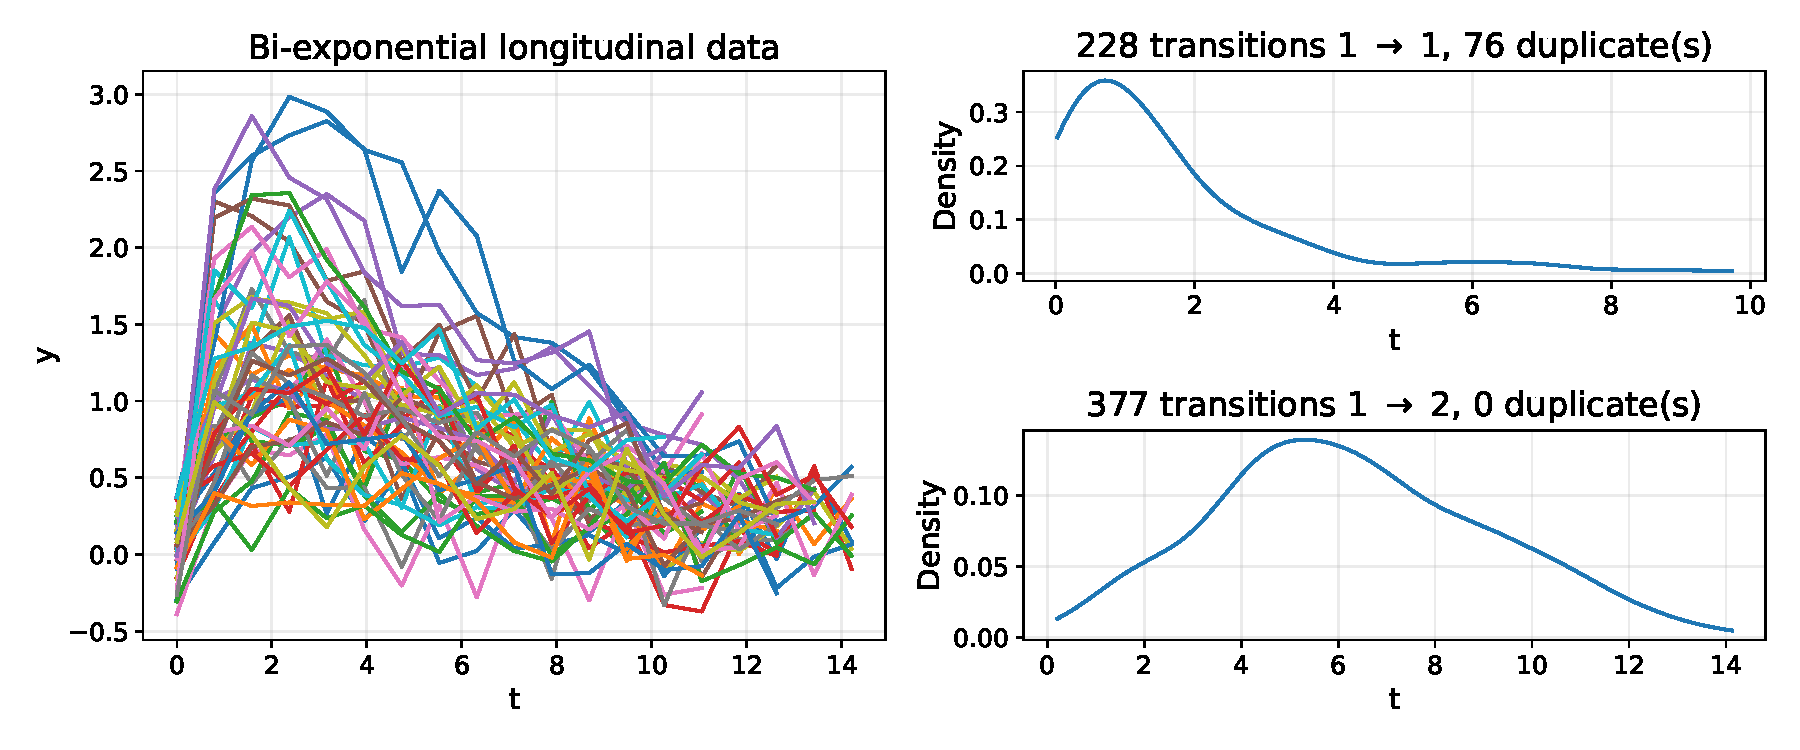
\includegraphics[width=\linewidth]{figures/simulated-sample.pdf}
    \end{minipage}
    \begin{minipage}{0.45\textwidth}
        \centering
        \begin{tabular}{|c|c|}
            \hline
            \textbf{From $\rightarrow$ To} & \textbf{\# Observations} \\
            \hline
            $0 \rightarrow 1$              & 613                      \\
            $0 \rightarrow 2$              & 375                      \\
            $1 \rightarrow 2$              & 592                      \\
            \hline
        \end{tabular}
    \end{minipage}
    \caption{Simulated data: on the left, a sample of longitudinal measurements from $50$ individuals; on the right, observed transitions between states for the complete population of $1000$ individuals.}
    \label{fig:simulation}
\end{figure}

\subsection{Estimator Convergence}

To illustrate the convergence of the estimator, we examine the optimization process for a particular run with $n = 1000$ (see Figure~\ref{fig:fitting-plots}), as well as RMSE values computed from $n_\text{runs} = 100$ independent runs on different simulated datasets, all generated from the same underlying distribution. The results of these simulations are shown in Table
\ref{tbl:convergence-rmse}.

To fit the model, we first have to define initial parameters, which can be particularly important for the optimization process if the model is not well-behaved. In the present case, without prior knowledge of the true parameters, we zero the values and use the identity matrix for both covariance matrices.

Formally, for any $t \geq 1$ and $i \in \{ 1, 2 \}$, consider
\[
    m_i^{(t)} \gets \beta_i m_i^{(t-1)} + (1 - \beta_i) (\theta^{(t)} - \theta^{(t-1)})^i, \quad \hat{m}_i^{(t)} = \frac{m_i^{(t)}}{1 - \beta_i^t},
\]
and the optimization process is terminated when
\[
    \vert \hat{m}_1^{(t)} \vert \leq 10^{-6} + 10^{-1} \sqrt{\hat{m}_2^{(t)}}.
\]

The Figure \ref{fig:fitting-plots} shows the evolution of the parameters during the optimization process, and Table~\ref{tbl:convergence-rmse} summarizes the accuracy of the inferred parameters.

\begin{figure}[H]
    \centering
    \begin{tabular}{lcccc}
        \hline
        Parameter             & True value & Mean     & Standard error & RMSE   \\
        \hline
        $\gamma_1$            & 2.5000     & 2.4960   & 0.0370         & 0.0372 \\
        $\gamma_2$            & -1.3000    & -1.3039  & 0.0257         & 0.0260 \\
        $\gamma_3$            & 0.2000     & 0.1936   & 0.0267         & 0.0275 \\
        $\tilde{Q}_1$         & 0.2554     & 0.2243   & 0.0442         & 0.0540 \\
        $\tilde{Q}_2$         & 0.8047     & 0.8009   & 0.0260         & 0.0263 \\
        $\tilde{Q}_3$         & 0.6020     & 0.6001   & 0.0276         & 0.0277 \\
        $\tilde{R}$           & -0.2653    & -0.2684  & 0.0083         & 0.0089 \\
        $\alpha_1^{1 \mid 0}$ & -0.5000    & -0.49997 & 0.0486         & 0.0486 \\
        $\alpha_2^{1 \mid 0}$ & -3.0000    & -2.9962  & 0.0800         & 0.0801 \\
        $\alpha_1^{2 \mid 0}$ & -1.0000    & -0.9990  & 0.0847         & 0.0847 \\
        $\alpha_2^{2 \mid 0}$ & -5.0000    & -4.9897  & 0.1191         & 0.1196 \\
        $\alpha_1^{2 \mid 1}$ & 0.0000     & 0.0011   & 0.0327         & 0.0327 \\
        $\alpha_2^{2 \mid 1}$ & -1.2000    & -1.2045  & 0.0429         & 0.0432 \\
        $\beta^{1 \mid 0}$    & -1.3000    & -1.3015  & 0.0501         & 0.0501 \\
        $\beta^{2 \mid 0}$    & -0.9000    & -0.8982  & 0.0670         & 0.0670 \\
        $\beta^{2 \mid 1}$    & -0.7000    & -0.6981  & 0.0551         & 0.0551 \\
        \hline
    \end{tabular}
    \caption{Comparison of true and estimated parameters (averaged over 100 runs).}
    \label{tbl:convergence-rmse}
\end{figure}

The simulation confirms that the proposed inference method accurately recovers all parameters of the multi-state joint model under realistic sample sizes. The optimization demonstrates stable convergence (Figure~\ref{fig:fitting-plots}), with minimal sensitivity to initialization. The algorithm’s computational efficiency allows for extensive simulation or cross-validation studies at negligible cost.

\section{Application to the PAQUID Cohort} \label{sec:paquid}

\subsection{Introduction}

The data used in this section originates from the PAQUID cohort
\citep{Letenneur1994}, a large prospective population-based study initiated in southwestern France in 1988, aimed at understanding the determinants and trajectories of aging. A subsample of $n = 500$ individuals was followed over a period of up to $20$ years \citep{Proust-Lima2017}, with repeated measures of cognitive and physical health, as well as socio-demographic characteristics. In particular, global cognitive functioning was assessed through the Mini-Mental State Examination (MMSE, see Figure~\ref{fig:paquid}), while physical dependency was evaluated using the HIER scale, which classifies subjects into four ordered states (see Figure~\ref{fig:hier-graph}): $0$ (no dependency), $1$ (mild dependency), $2$ (moderate dependency), and $3$ (severe dependency). In this work, we focus on the association between cognitive decline and the progression of physical dependency by jointly modeling the longitudinal trajectory of MMSE scores and the transitions between the four HIER states using a joint multi-state model. More specifically, the state of an individual at a given time $t$ is defined as the highest HIER dependency score between trial entry and $t$. This approach allows us to characterize the dynamic interrelationship between cognitive and physical aging processes within a unified statistical framework.

Both time and longitudinal values were normalized in $[-1, 1]$. This technique ensured stable and fast convergence of the optimization process by keeping all parameters on roughly the same scale.

\begin{figure}[H]
    \centering
    \begin{minipage}{0.5\textwidth}
        \centering
        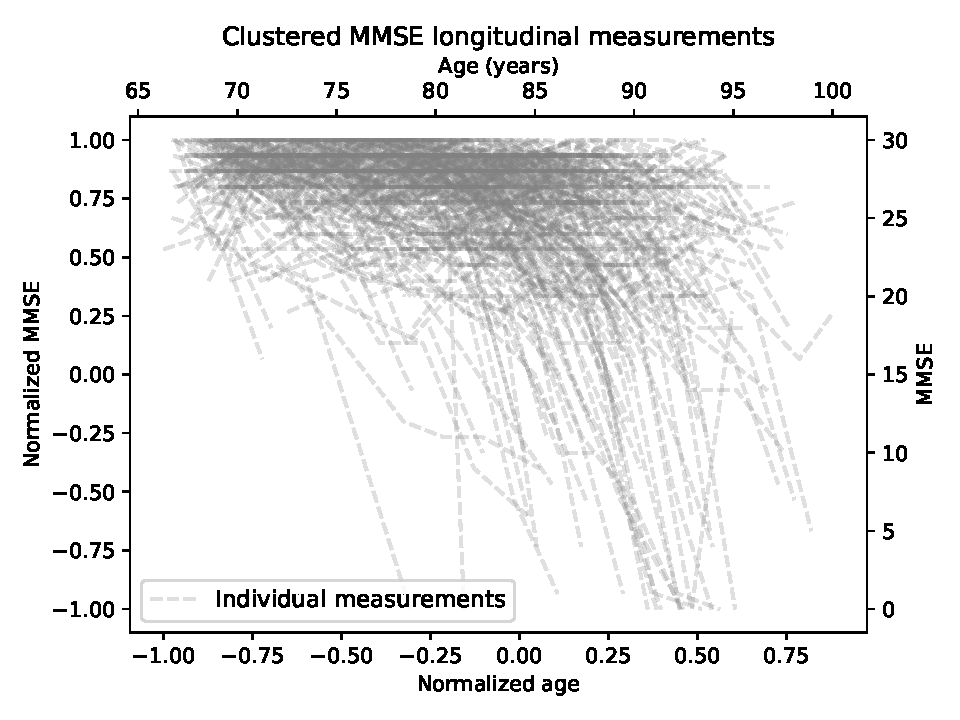
\includegraphics[width=\linewidth]{figures/paquid-mmse.pdf}
    \end{minipage}
    \begin{minipage}{0.45\textwidth}
        \centering
        \begin{tabular}{|c|c|}
            \hline
            \textbf{From $\rightarrow$ To} & \textbf{\# Observations} \\
            \hline
            $0 \rightarrow 1$              & 85                       \\
            $1 \rightarrow 2$              & 135                      \\
            $2 \rightarrow 3$              & 86                       \\
            $0 \rightarrow 2$              & 44                       \\
            $1 \rightarrow 3$              & 15                       \\
            $0 \rightarrow 3$              & 11                       \\
            \hline
        \end{tabular}
    \end{minipage}
    \caption{On the left, each light gray line represents one of the $500$ observed sequences of (normalized) MMSE scores, and three functional clusters are also represented; on the right, observed transitions between states.}
    \label{fig:paquid}
\end{figure}

Therefore, the chosen transition graph is as follows, and only allows monotonic transitions from a lower level of physical dependency to a higher one.

\begin{figure}[H]
    \centering
    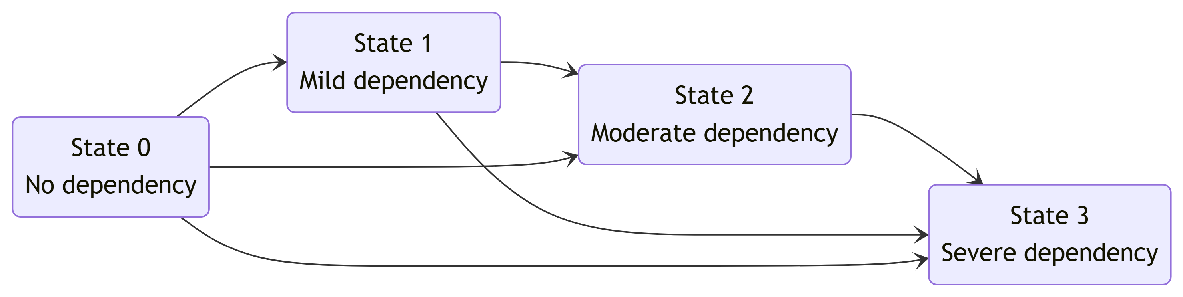
\includegraphics[width=0.8\textwidth]{diagrams/hier-graph.pdf}
    \caption{Schematic representation of the four ordered HIER states, with possible transitions. HIER quantifies physical dependency ($0$: no dependency to $3$: severe dependency) \citep{Proust-Lima2017}.}
    \label{fig:hier-graph}
\end{figure}

We consider an exponential baseline hazard model for transitions, with a \emph{clock reset} specification. The parameters of these exponential baseline hazards are jointly optimized with the model parameters.

Moreover, we impose a particular substructure on the model, where $\forall (k, k') \in E, \, \beta^{k' \mid k} = \beta$.

In the light of Figure~\ref{fig:paquid}, the regression and link
functions were taken to be scaled and shifted hyperbolic tangent and its derivative respectively such that the normalized MMSE score always has a value of $1$ when $t \to -\infty$ and is not increasing
\[
    \begin{cases}
        h(t, \psi) = \psi_1 \tanh\left(\frac{\psi_3 - t}{\psi_2}\right) + (1 - \psi_1), \\
        g(t, \psi) = \frac{\partial}{\partial t} h, \\ 
        \psi =
        \begin{pmatrix}
            \sigma(\gamma_1 + b_1) \\
            \exp(\gamma_2 + b_2)   \\
            \gamma_3 + b_3
        \end{pmatrix}, \quad \sigma(z) = \frac{1}{1 + e^{-z}}.
    \end{cases}
\]

At last, individual covariates correspond to a pair of binary variables indicating whether or not the individual has a diploma and is a male $\left(\mathds{1}_\text{CEP}(i), \mathds{1}_\text{male}(i)\right) \in \{0, 1\}^2$.

\subsection{Results}

\subsubsection{Inference}

Fitting was performed using $80\%$ of the data, with the remaining $20\%$ used for testing. The model was fitted using the Adam optimizer. The optimization process was run until convergence based on the same criterion as the simulation study with a tolerance of $5\%$, which was obtained after a little less than $500$ iterations with $10$ parallel chains.

Before displaying the fitted parameters, the Fisher Information Matrix was computed, implementing the method described in \cite{baey2023efficient}, directly taking into account shared parameters. The standard errors were then computed as the square root of the diagonal of the inverse of the Fisher Information Matrix. The results are summarized in Table~\ref{tbl:paquid-fit}.

\begin{figure}[H]
    \centering
    \begin{tabular}{lcc|lcc}
        \hline
        Parameter & Inferred value & Std. error & Parameter & Inferred value & Std. error \\
        \hline
        $\gamma_1$ & \textbf{2.1600} & \textbf{0.0470} & $\gamma_2$ & \textbf{0.1590} & \textbf{0.0140} \\
        $\gamma_3$ & \textbf{1.0010} & \textbf{0.0030} & $\tilde{Q}_1$ & \textbf{-0.5700} & 0.0430 \\
        $\tilde{Q}_2$ & 0.9570 & 0.0960 & $\tilde{Q}_3$ & 0.3820 & 0.0430 \\
        $\tilde{Q}_4$ & -0.2050 & 0.1570 & $\tilde{Q}_5$ & \textbf{-2.3310} & \textbf{0.1380} \\
        $\tilde{Q}_6$ & 0.5220 & 0.0470 & $\tilde{R}$ & \textbf{2.0830} & \textbf{0.0260} \\
        $\alpha^{3 \mid 1}$ & 0.7220 & 0.7150 & $\alpha^{1 \mid 0}$ & -0.5400 & 0.4030 \\
        $\alpha^{2 \mid 1}$ & \textbf{-1.0030} & \textbf{0.2000} & $\alpha^{2 \mid 0}$ & \textbf{-0.1210} & \textbf{0.0380} \\
        $\alpha^{3 \mid 2}$ &  -0.0480 & 0.2520 & $\alpha^{3 \mid 0}$ & \textbf{-0.3070} & \textbf{0.0740} \\
        $\beta_1$ & -0.2990 & 0.9130 & $\beta_2$ & 0.0970 & 1.0300 \\
        \hline
    \end{tabular}
    \caption{Inferred parameters and their estimated standard deviations. Bold values mean $p < 0.05$ (variance parameters excluded).}
    \label{tbl:paquid-fit}
\end{figure}

Notably, the estimated standard errors are consistent with the number of observations per transition, with larger standard errors for transitions with fewer observations. Therefore, parameters with too few observations should be interpreted with caution, if at all. The linear covariate parameters also exhibit large standard errors, which indicates the coefficients are not statistically significant in this setting.

The negative values of the association parameters $\alpha$ suggest that greater cognitive decline is associated with a higher rate of progression in physical dependency.

\subsubsection{Dynamic Prediction}

Using the $n_\text{test} = 100$ individuals not included in the model fitting, we performed dynamic prediction through a single Monte Carlo integration scheme as defined in Section~\ref{sec:prediction}. For each individual, longitudinal measurements and trajectories were truncated at various times $t$, and predictions were made for future time points $u \geq t$ beyond the truncation. Accuracy was then assessed by comparing the most likely predicted state with the true state at each corresponding future time point $u$, as illustrated in Figure~\ref{fig:paquid-acc}.

Formally, the prediction function $\chi_u^*$ is defined by Example
\ref{ex:state-at-time-u}, and the accuracy measure at time $t$ for predicted states $(s_i)_i$ is defined as
\[
    \text{accuracy}(u) = \frac{1}{n_\text{test}} \sum_{i=1}^{n_\text{test}} \mathds{1}_{\chi_{u \wedge C_i}(\mathcal{T}_i) = s_i}.
\]

Although $\mathcal{T}_i^*$ is unknown, the quantity $\chi_{u \wedge C_i}(\mathcal{T}_i)$ may be computed based on the censored trajectories. However, incorporating censoring times into prediction functions relies on information that is, in principle, not available at prediction time. Nevertheless, this inclusion is necessary to ensure fairness in accuracy metrics, since individuals who are not censored are generally more likely to have progressed to more advanced states of physical dependency than those who are censored.

\begin{minipage}{0.5\textwidth}
    \begin{figure}[H]
        \centering
        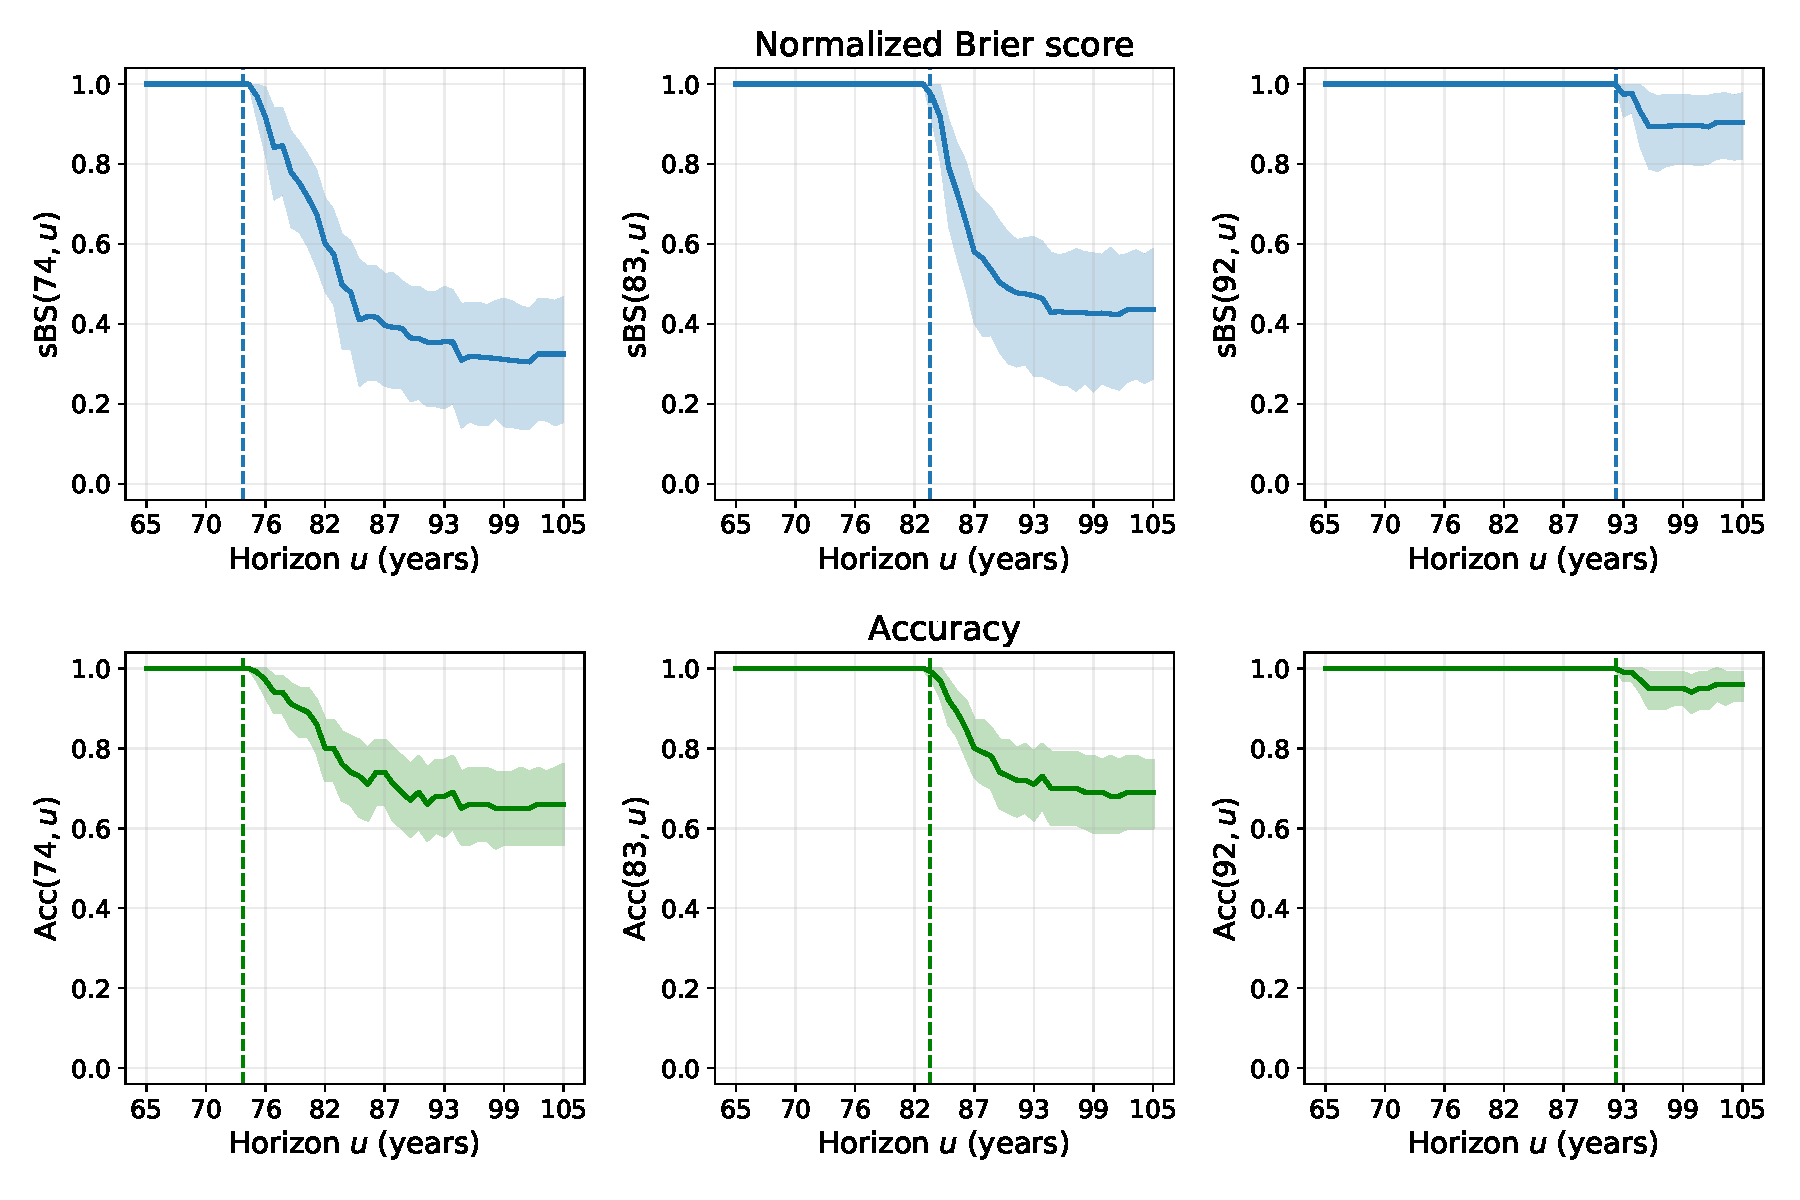
\includegraphics[width=\textwidth]{figures/paquid-accuracy.pdf}
        \caption{Accuracy of the predicted state at each time point with respect to the true state for different truncation times.}
        \label{fig:paquid-acc}
    \end{figure}
\end{minipage}
\hfill
\begin{minipage}{0.45\textwidth}
    Here, the initial drops correspond to the truncation times, before which the accuracy is always $100\%$.

    \bigbreak

    As expected from dynamic predictions, the accuracy increases as more data is available, therefore when the truncation time grows. We also observe that the longer the prediction horizon, the lower the accuracy of the predictions.

\end{minipage}

\section{Conclusion} \label{sec:conclusion}

We presented a general likelihood-based framework for joint modeling of nonlinear longitudinal biomarkers and multi-state survival processes. The model unifies both components on arbitrary directed graphs, extending classical joint models to accommodate Markov and semi-Markov structures, recurrent transitions, and nonlinear mixed-effects submodels. This formulation provides a flexible and rigorous foundation for linking longitudinal biomarker trajectories to complex event histories within a single coherent probabilistic model.

Simulation studies confirmed robust parameter recovery, and an application to the PAQUID cohort highlighted the ability to capture the interplay between cognitive decline and physical dependency.

Since the model may potentially involve many transitions and therefore a large number of parameters, a strategy of parameter sharing across transitions could help reduce the overall number of parameters. This is especially beneficial in settings with limited data for certain transitions, or when biological or clinical knowledge suggests similar effects across multiple transitions. Parameter sharing improves statistical efficiency, reduces overfitting, and facilitates model interpretability.

Future directions include a spline-based parametrization of baseline hazards to allow for nonparametric estimation. This approach is particularly useful when the true baseline hazard is expected to be complex or non-monotonic, or when parametric forms (such as exponential or Weibull) may be too restrictive and lead to model misspecification.

Another promising direction is the development of efficient visualization tools for multi-state trajectories and dynamic predictions. Interactive representations of individual event histories, transition probabilities, and longitudinal biomarker evolution would greatly facilitate model interpretation and communication of results to applied researchers.

\section*{Funding}

This work was partially funded by the Stat4Plant project
ANR-20-CE45-0012.

\section*{Acknowledgments}

The authors would like to thank Jean-Benoist Leger for helpful
discussions.

\subsection*{Conflict of interest}
The authors declare that they have no conflicts of interest.


\subsection*{Data availability}
The data analyzed in this study are publicly available via the R package \texttt{timeROC} (dataset \texttt{Paquid}).

\bibliographystyle{sn-basic}
\bibliography{sources}

\appendix

\section{Multi-State Simulation}

In nonlinear joint models with known design and known parameters
parameters $\theta = (\gamma, Q, R, \alpha, \beta)$, the occurrence times of events conditionally on the latent variables $b_i$ and the covariates $X_i$ can be easily sampled using the inverse cumulative distribution function transform method. This may be achieved through bisection or other root-finding algorithms.

The simulation of the transition process $\mathcal{T}_i^*$ conditionally on $b_i$, $X_i$, and $(T_{i0}, S_{i0})$ can be achieved drawing on the semi-Markov property  by considering one transition at a time, according to Algorithm~\ref{alg:trajectory-sim}. The algorithme is similar to Gillespie's algorithm \citep{gillespie2007stochastic}, and can also include a survival condition $T_{i1} \geq t_i^\text{surv}$ that uses the Chasles relation.

\begin{algorithm}[H]
    \caption{Simulation of trajectory $i$}
    \label{alg:trajectory-sim}

    \begin{algorithmic}[1]
        \renewcommand{\algorithmicrequire}{\textbf{Input:}}
        \Require subject-specific censoring time $C_i \in \mathbb{R} \cup \{ +\infty \}$; covariates $X_i$; latent variables $b_i$; initial time-state pair $(T_{i0}, S_{i0})$; optional survival condition $T_{i1} \geq t_i^\text{surv}$, defaults to $t_i^\text{surv} = -\infty$.
        \Statex
        \State Initialize $\ell_i \gets 1$, $\mathcal{T}_i \gets \left( (T_{i0}, S_{i0}) \right)$.
        \Statex
        \While{$T_{i(\ell_i-1)} < C_i$ and $\{ s: (S_{i(\ell_i-1)}, s) \in E \} \neq \emptyset$}
        \For{each $s$ with $(S_{i(\ell_i-1)}, s) \in E$}
        \State Draw $T_{i\ell_i}^s$ such that
        \Statex \hspace{\algorithmicindent} \hspace{\algorithmicindent} $-\log \mathbb{P}(T_{i\ell_i}^s > t) = \int_{T_{i(\ell_i-1)} \vee t_i^\text{surv}}^t \lambda_i^{s \mid S_{i(\ell_i-1)}}(w \mid b_i, X_i, T_{i(\ell_i-1)}, \theta)\, dw,$
        \Statex \hspace{\algorithmicindent} \hspace{\algorithmicindent} $\forall t \geq T_{i(\ell_i-1)} \vee u.$
        \EndFor
        \Statex
        \State Set $T_{i\ell_i} \gets \min_m T_{i\ell_i}^s$, and $S_{i\ell_i} \gets \arg \min_m T_{i\ell_i}^s$.
        \State Append $(T_{i\ell_i}, S_{i\ell_i})$ to $\mathcal{T}_i$.
        \State $\ell_i \gets \ell_i + 1$.
        \EndWhile
        \Statex
        \If{$T_{i(\ell_i-1)} > C_i$}
        \State Remove the last pair: $\mathcal{T}_i \gets \mathcal{T}_i[:-1]$.
        \EndIf
        \State \Return $\mathcal{T}_i$
    \end{algorithmic}
\end{algorithm}

The proof of the exactness of this algorithm is given below.

\begin{proof}
    First consider the case $t_i^\text{surv} = -\infty$. Let $t > T_{i\ell_i}$. One has
    \begin{align*}
        \mathbb{P}(T_{i(\ell_i+1)} > t \mid T_{i\ell_i}, S_{i\ell_i}) &= \mathbb{P}(\bigcap_{s : \, (E_{i(\ell_i-1)}, s) \in E} T_{i(\ell_i+1)}^s > t \mid T_{i\ell_i}, S_{i\ell_i}), \\
        &= \prod_{s : \, (S_{i\ell_i}, s) \in E} \mathbb{P}(T_{i(\ell_i+1)}^s > t \mid T_{i\ell_i}, S_{i\ell_i}), \\
        &= \exp \Big(-\sum_{s : \, (S_{i\ell_i}, s) \in E} \Lambda_i^{s \mid S_{i(\ell_i-1)}}\big(t \mid b_i, X_i, T_{i\ell_i}, \theta)\Big).
    \end{align*}
    
    Furthermore
    \begin{align*}
        & \mathbb{P}(S_{i(\ell_i+1)} \mid T_{i(\ell_i+1)} = t, T_{i\ell_i}, S_{i\ell_i}) \\
         & \propto p(\{ T_{i(\ell_i+1)}^{S_{i(\ell_i+1)}} = t \} \cap \bigcap_{\substack{s : \, (S_{i\ell_i}, s) \in E, \\ s \neq S_{i(\ell_i+1)}}} \{ T_{i(\ell_i+1)}^s \geq t \} \mid T_{i\ell_i}, S_{i\ell_i}), \\
         & = \lambda_i^{S_{i(\ell_i+1)} \mid S_{i\ell_i}}\big(t \mid \theta, X_i, T_{i\ell_i}, b_i) \exp \Big(-\sum_{s : \, (S_{i\ell_i}, s) \in E} \Lambda_i^{s \mid S_{i\ell_i}}\big(t \mid b_i, X_i, T_{i\ell_i}, \theta)\Big).
    \end{align*}

    Combining both, we retrieve the same joint density.

    If $t_i^\text{surv} > -\infty$, one can also check that both densities are equal. Note that the condtioning only affects the first transition, as the next time $\forall \ell_i > 0, \, T_{i\ell_i} \geq t_i^\text{surv} \implies \forall \ell_i > 0, \, T_{i\ell_i} \vee t_i^\text{surv} = T_{i\ell_i}$.

\end{proof}

\section{Expression of the Semi-Markov likelihood} \label{sec:proof-semi-markov}

\begin{proof}

    The proof is short and relies on the fact that, using the semi-Markov property~\ref{ass:semi-markov}
    \begin{align*}
    p\left((T_{i(\ell+1)}, S_{i(\ell+1)})_{\ell \leq m_i - 1} \mid b_i, X_i, \theta\right) & = \prod_{\ell=0}^{m_i - 1} p\left((T_{i(\ell+1)}, S_{i(\ell+1)}) \mid b_i, X_i, (T_{i\ell'}, S_{i\ell'})_{\ell' \leq \ell}, \theta\right), \\
    &= \prod_{\ell=0}^{m_i - 1} p\left((T_{i(\ell+1)}, S_{i(\ell+1)}) \mid b_i, X_i, (T_{i\ell}, S_{i\ell}), \theta\right).
    \end{align*}

    On the other hand, the probability that no additional event is observed between $T_{im_i}$ and $C_i$ is $1$ if the last state reached is absorbing, and otherwise
    \[
        \mathbb{P}(T_{i (m_i+1)} > C_i \mid \theta, X_i, (T_{im_i}, S_{im_i}), b_i) = \exp\left(-\sum_{s : \, (S_{im_i}, s) \in E} \Lambda_i^{s \mid S_{im_i}}(C_i \mid b_i, X_i, T_{im_i}, \theta)\right),
    \]
    and so we recover the formula cited above with the convention that an empty sum is $0$.

\end{proof}

\section{Stochastic optimization process}

\begin{figure}[H]
    \centering
    \vspace{-1.7em}
    \begin{subfigure}{0.3\textwidth}
        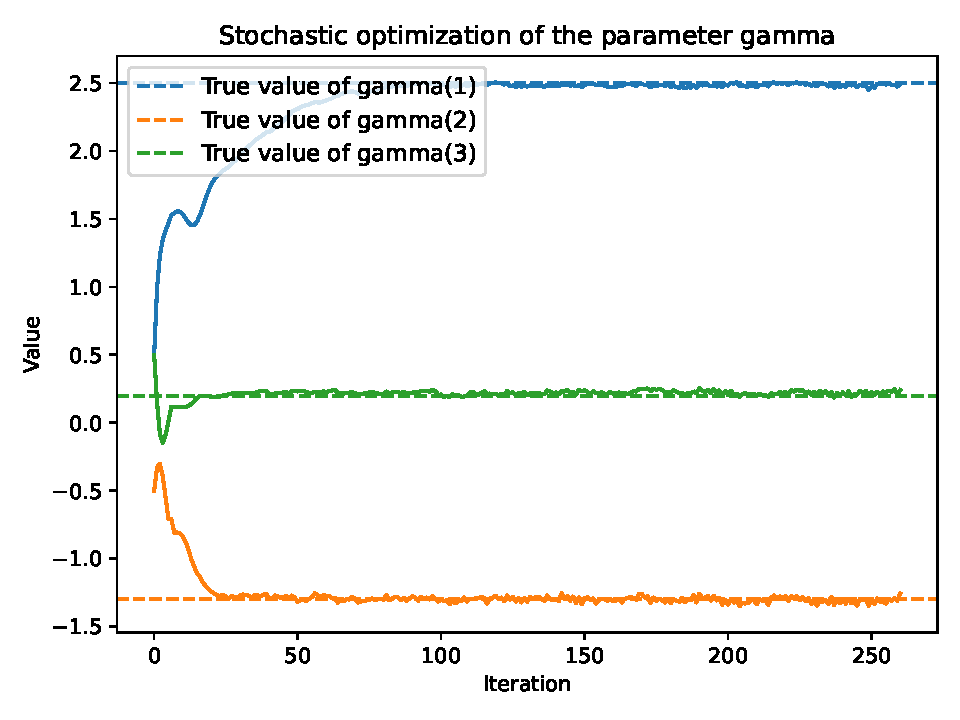
\includegraphics[width=0.99\linewidth]{figures/gamma.pdf}
        \caption{$\gamma$}
    \end{subfigure}
    \hfill
    \begin{subfigure}{0.3\textwidth}
        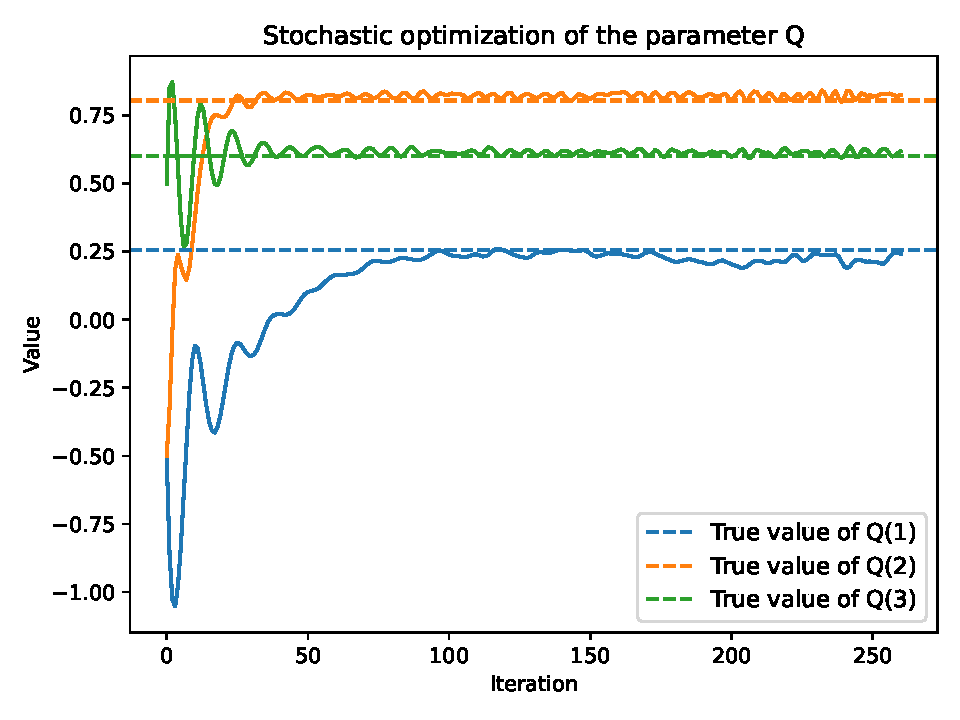
\includegraphics[width=0.99\linewidth]{figures/Q.pdf}
        \caption{$Q$}
    \end{subfigure}
    \hfill
    \begin{subfigure}{0.3\textwidth}
        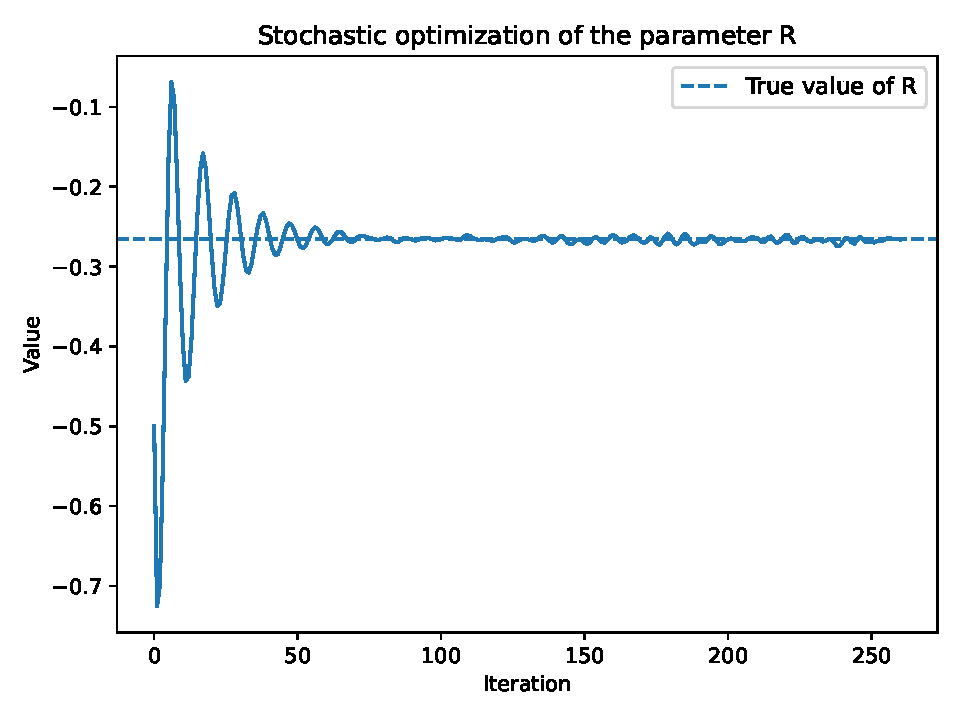
\includegraphics[width=0.99\linewidth]{figures/R.pdf}
        \caption{$R$}
    \end{subfigure}
    \\[-0.3em]
    \begin{subfigure}{0.3\textwidth}
        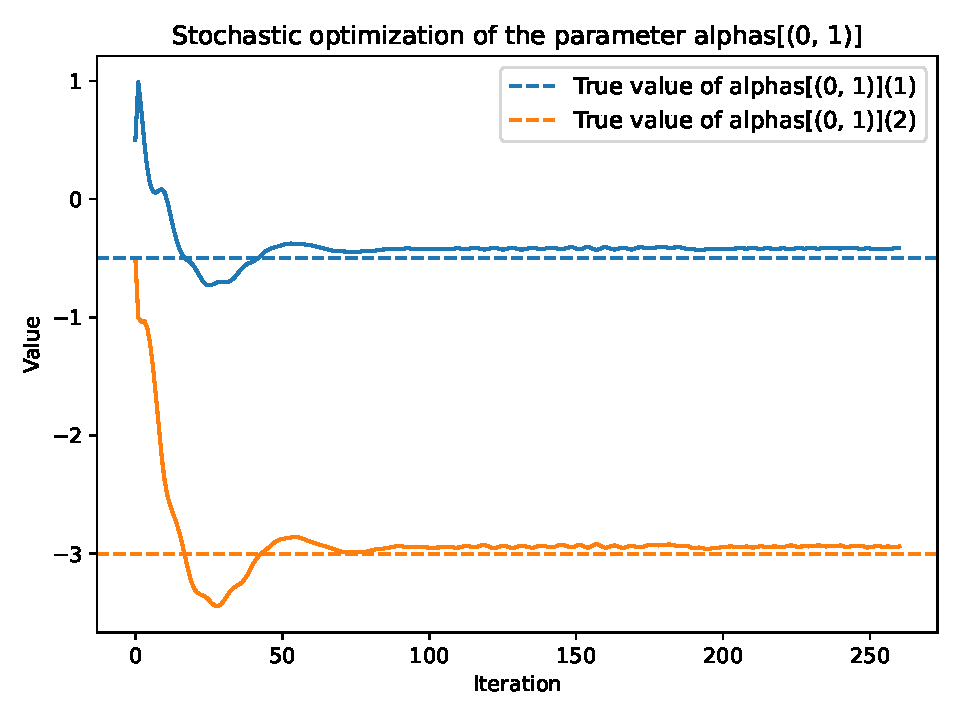
\includegraphics[width=0.99\linewidth]{figures/alphas01.pdf}
        \caption{$\alpha^{1 \mid 0}$}
    \end{subfigure}
    \hfill
    \begin{subfigure}{0.3\textwidth}
        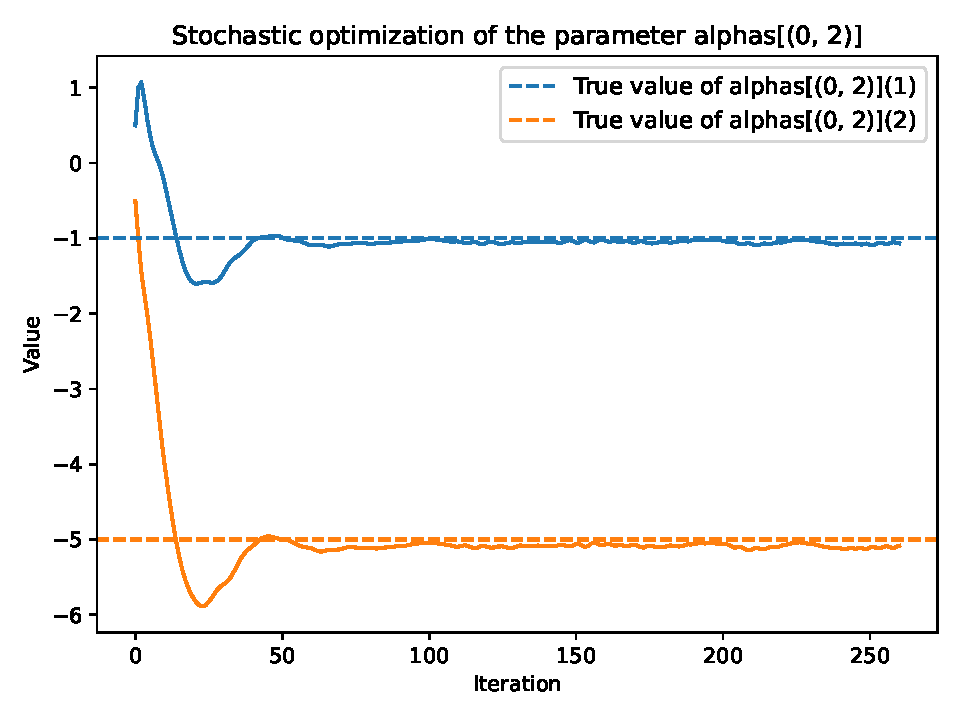
\includegraphics[width=0.99\linewidth]{figures/alphas02.pdf}
        \caption{$\alpha^{2 \mid 0}$}
    \end{subfigure}
    \hfill
    \begin{subfigure}{0.3\textwidth}
        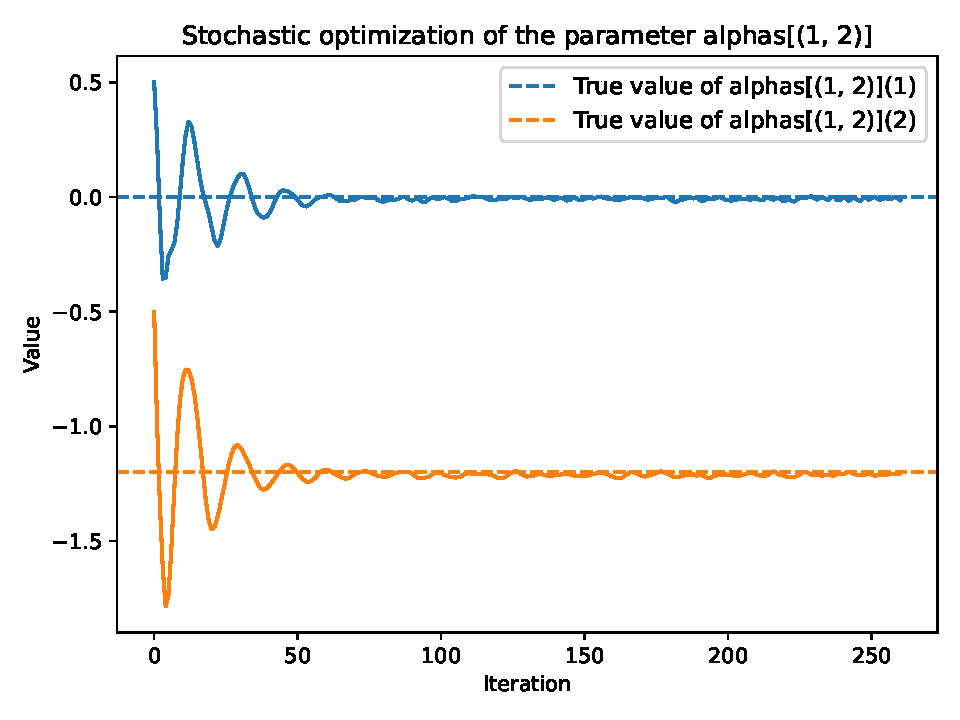
\includegraphics[width=0.99\linewidth]{figures/alphas12.pdf}
        \caption{$\alpha^{2 \mid 1}$}
    \end{subfigure}
    \\[-0.3em]
    \begin{subfigure}{0.3\textwidth}
        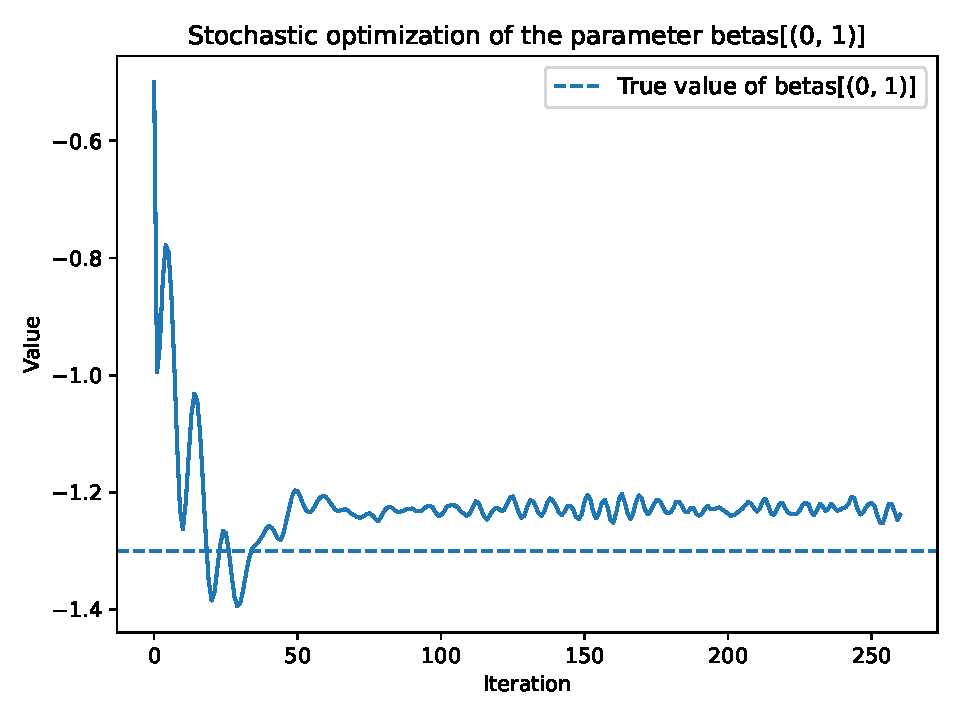
\includegraphics[width=0.99\linewidth]{figures/betas01.pdf}
        \caption{$\beta^{1 \mid 0}$}
    \end{subfigure}
    \hfill
    \begin{subfigure}{0.3\textwidth}
        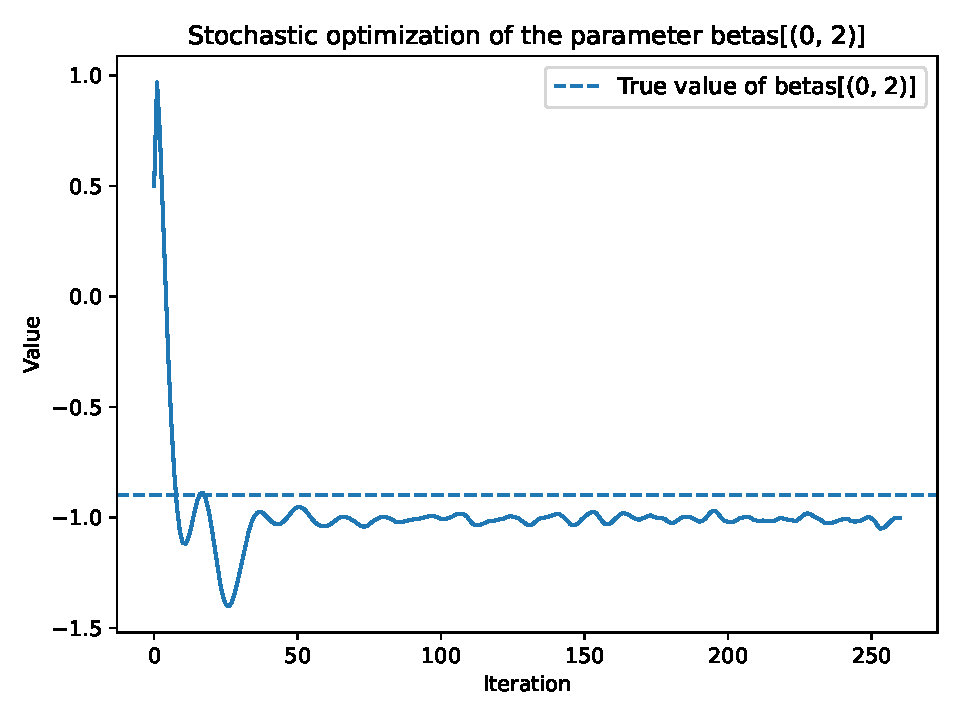
\includegraphics[width=0.99\linewidth]{figures/betas02.pdf}
        \caption{$\beta^{2 \mid 0}$}
    \end{subfigure}
    \hfill
    \begin{subfigure}{0.3\textwidth}
        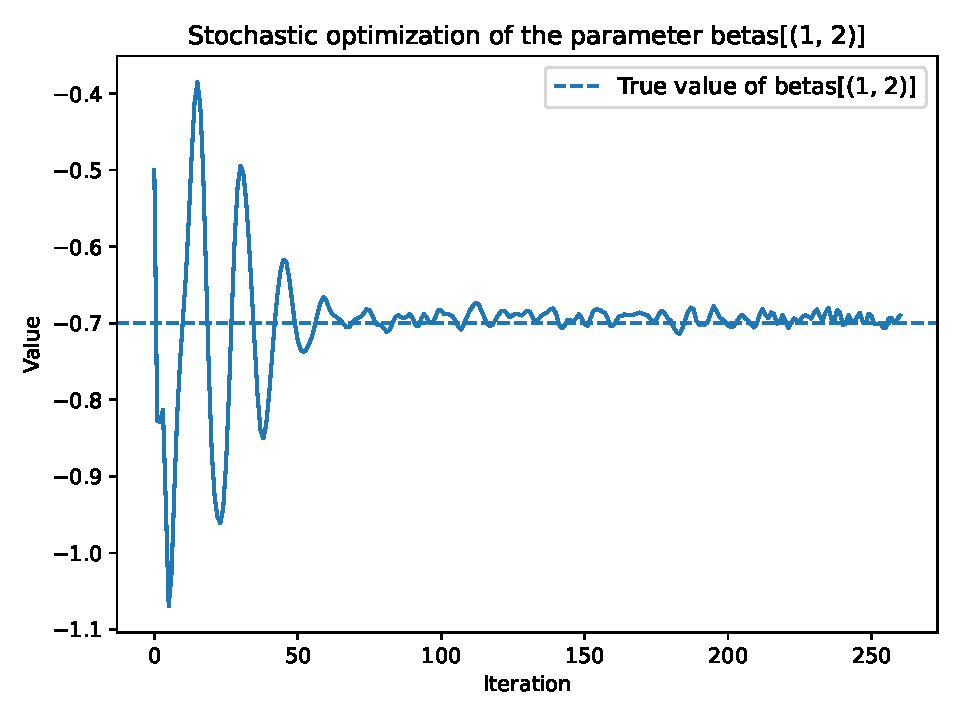
\includegraphics[width=0.99\linewidth]{figures/betas12.pdf}
        \caption{$\beta^{2 \mid 1}$}
    \end{subfigure}

    \caption{Evolution of the parameters during the optimization of the marginal log-likelihood using stochastic gradient descent. The dotted lines correspond to the true values.}
    \label{fig:fitting-plots}
\end{figure}

\end{document}
